\documentclass{scrartcl}
\usepackage[utf8]{inputenc}
\usepackage{amsmath}
\usepackage{graphicx}
\setlength{\parindent}{0ex}
\usepackage{booktabs}
\usepackage{caption}


\usepackage[
%  style=authoryear,
%  maxcitenames=1,
%  maxbibnames=99
  natbib=true,
  backend=bibtex
]{biblatex}
\addbibresource{literatur.bib}

\setlength{\bibitemsep}{0.5\baselineskip}

\usepackage{longtable}
\usepackage{amssymb}
\usepackage{hyperref}
\usepackage[ruled,noline]{algorithm2e}
\providecommand{\SetAlgoLined}{\SetLine}
\providecommand{\DontPrintSemicolon}{\dontprintsemicolon}
\usepackage[left=2cm,right=2cm,top=1.3cm,bottom=2.2cm]{geometry}

\usepackage{setspace}
\onehalfspacing

\usepackage{subfigure}


\DeclareCaptionFormat{upper}{#1#2\uppercase{#3}\par}
\renewcommand{\thesubfigure}{\Alph{subfigure}}


\newenvironment{items}{
\begin{itemize}
  \setlength{\itemsep}{1pt}
  \setlength{\parskip}{0pt}
  \setlength{\parsep}{0pt}
}{\end{itemize}}

\title{\texttt{BacArena}: Simulation of Interactions in Microbial Communities using Genome-wide Metabolic Reconstructions}
\author{Johannes Zimmermann\\Eugen Bauer}
\date{\today}

\begin{document}

\maketitle

\section*{Abstract}
Microbial communities are essential for global ecosystems and human health.
Computational modeling of microbial consortia is thus a major goal in systems biology and microbial ecology. 

\texttt{BacArena} is a project to simulate bacterial behaviour in communities. A lot of progress is done in the last years to gain genome wide metabolic reconstructions of certain organisms, which open a wide field of mathematical analysis.
One of this new methods is flux balanced analysis (fba) to estimate optimal metabolic fluxes under certain constraints. By this work advanced models are possible, which are available in a defined, exchangeable format (\emph{SBML}). The idea of this project is to use this existing reconstructions and put them in a spatial and temporal environment to study their possible interactions.
This is achieved by the combination of agent based modeling with fba. Each bacterium is considered as an agent with individual states, own properties and rules to act. Agents are located on a grid where they can move and interact via metabolic exchanges computed by fba.

The starting point for our project is curiosity of what could be done with this huge models. We just throw those models into an arena to see what kind of actions will evolve.
\newpage

\tableofcontents

\newpage

\section{Introduction}
\subsection{Microbial metabolic ecology}
Microbial communities pose important roles in the cycle of matter ( *) as well as human health and disease ( *). The comprehensive understanding of the interaction between microbes is thus a major goal in microbial ecology and systems biology. 

Microbial consortia often consist of a diverse composition, which degrade complex compounds in multiple steps by different microbes ( *). This division of labour can be realized by the aggregation to biofilms in which multiple layers of microbes are associated with each other and interact by exchanging various metabolites ( *). An example for the cross-feeding between microbes is the interspecies hydrogen transfer. Here, methanogenic archea are associated with bacteria or protists, which produce hydrogen after anearobic degradation ( *). The hydrogen can be taken up as an essential substrate by the methogens, which profits the producer by the removal of the products and thus the thermodynamic limitation ( *). Therefore both partners benefit from this interaction. A close spatial aggregation of the partners can further optimize their individual benefits, since the hydrogen can be exchanged faster.

Recent advances in systems biology made it possible to study the metabolic interactions of multiple species on the systems level ( *). In particular constrained based modeling can be applied to model interspecies metabolic exchanges ( *).
 
\subsection{Constrained based modeling}
\label{cobra}
Constrained based modeling is a successfully applied method in systems biology (\cite{Esvelt2013}, \cite{Klipp2010} p. 353), where the metabolism of single species is considered as a network of biochemical reaction.
The reaction network itself can be represented more formally with differential equations using mass action kinetics.
Because of the high numbers of reactions and metabolites the resulting system of equation and the solution space is high dimensional.
Therefore, linear algebra is used for a simplified description:
\[
  \frac{dx}{dt}=S \cdot v
\]
where $x\in \mathbb{R}^m$ is a vector consisting of concentrations of all $m$ metabolites, $S\in \mathbb{Z}^{m\times r}$ is the stoichiometric matrix, which includes the net consumption/production of all $r$ biochemical reactions and $v \in \mathbb{R}^r$ is the flux vector which contains in general nonlinear kinetic relationships.

Now several \textit{constraints} could be applied to solve the problem more easily. The most prominent constraint is the equilibrium or steady state $dx/dt \stackrel{!}{=}0$.
It is a reasonable assumption for a metabolic model, because there is evidence for a metabolic steady state in general (i.e. no net change for every metabolites at each time point)(\cite{Harris1995} p. 10-11).

One important constrained based modeling approach is flux balance analysis (fba) (\cite{Varma1994}, \cite{Orth2010}), which will be of utmost importance for this project.
Here, the former nonlinear problem $dx/dt=S\cdot v$ diminishes to $dx/dt=S\cdot v \stackrel{!}{=}0$, which constitutes a normal linear equation systems.
Nevertheless, there are far more reactions than metabolites ($r>m$), so that this linear reaction system is underdetermined.
That is why other constraints like flux limits are added.
Flux limits are reaction limits, which narrow down each reaction to some intervall (e.g. irreversible reaction number $i$ has a flux $v_i>0$).
By this the solution space is shrinked.
If the biomass composition, non and growth associated maintenance (ngam/gam) is known, it is possible to formulate an optimization problem:
\begin{equation*}
  \begin{aligned}
    & \underset{v}{\text{maximize}} & & b(v) \\
    & \text{subject to} & & S \cdot v = 0 \\
    & & & l_i < v_i < u_i
  \end{aligned}
\end{equation*}
where $l_i$ and $u_i$ are the lower and upper limits for reaction $i$ and $b(v)$ is biomass function, which is going to be maximized with respect to a certain flux $v$.
Thus, we search a vector $v$ carrying quantitative values for all fluxes in the whole reaction system, so that a certain function (here biomass function) is optimal. Although constrained based modeling frameworks for studying species interactions exist ( *), the complexity of microbial communities is still difficult to asses with this approaches.

\subsection{Agent based modeling}
\textit{Complexity theory} is a part of system science since 1970s, where order is not longer considered as something given but made by itself. Moreover, order is producible as a surface phenomenon by a complex process, which is i) self organizing, ii) secures its autonomity and iii) proceeds far from an equilibrium (\cite{Cilliers2007} p. 8-10).

According to John Holland, who introduced the important notion of an \textit{agent}, a complex adaptive system (CAS) is defined as follows:
\begin{quote}
,,We will view CAS as systems composed of interacting agents described in terms of rules. These agents adapt by changing their rules as experience accumulates.'' (\cite{Holland1995} p. 10)
\end{quote}
In this modeling paradigm no general differential equation governs the macro behaviour.
The parts of the system called agents are explicitly described by \textit{rules} instead of a theory.
This enables the possibility to model ,,microscopic'' phenomenons, which give individual properties and defined information to the agents.
,,If-then rules'' are heuristic and could depict relationships, where no mathematical description exists.
Therefore, agents have individuality, live in a surrounding area (grid) with limited radius, so that only local interactions in the neighbourhood governed by rules are relevant to produce a global phenomenons.

From this microscopic actions the global organization is produced.
New properties and behaviour could occur and this is noted by the slightly magical term \textit{emergence} (\cite{Zimmermann2010} p. 36-39).

Agent based modeling (abm) has been successfully applied in ecological studies to model the complexity of global behaviours by simple local interactions between species ( *).

\subsection{Aim of the project}
The aim of this project is to combine for the first time constrained based modeling in an ecological context with abm to model interactions in microbial communities. In particular microbes are represented as agents which interact with their surrounding substrate concentrations stored in a grid. These interactions are realized with fba, which is used as a rule.

This framework will be used to represent common observations in microbial ecology such as syntrophy.
%The whole is more than the sum of its parts. [Aristotle]...


\section{Methods}
\subsection{Model overview}
To model the metabolic the interaction of multiple species populations, each individual was represented as an agent on a grid environment (Figure \hyperref[fig:bacarena]{\ref{fig:bacarena}}).
\begin{figure}[h!]\centering
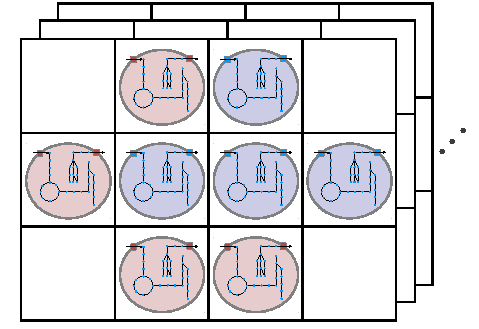
\includegraphics[scale=1.4]{method_chart_BacArena.pdf}
\caption[Overview BacArena]{Overview of the grid environment with two different bacterial agent types (species) in red and blue. Each substrates has its own grid representation.}
\label{fig:bacarena}
\end{figure}
The grid environment was composed of different metabolite concentrations.
Furthermore, the species type was recorded for each agent to call the respective genome-wide metabolic reconstruction in every iteration (Algorithm \hyperref[alg:mainloop]{\ref{alg:mainloop}}). The constraints for the subsequent fba were set according to the current metabolite concentrations of the grid cell, where the respective agent was located.
\begin{algorithm}
\caption{Main model iterations called by \texttt{diffbac.R} with the different functions applied to bacterial agents and metabolite concentrations.}
\SetAlgoLined
\For{number of iterations}{
  \emph{diffusion}()\;
  \For{number of bacteria}{
    \emph{fba}()\;
    \emph{movement}()\;
    \emph{growth}()\;
  }
}
\label{alg:mainloop}
\end{algorithm}
The solution of the fba was used to adjust the biomass of each agent and to modify the metabolite concentrations according to the produced products and consumed substrates. 
This uptake and output of metabolites constitute the exchange with the virtual environment.
A diffusion model was applied to spread the metabolite concentrations over the grid environment and a movement function allowed the random dispersal of each bacterial agent.

A central theme of \texttt{BacArena} was the modularity of each funcsubtion and metabolic model to allow the extension and replacement of certain parts of the framework. Furthermore, the modularity also enables the inclusion of any desired amount of microbial species. In the following sections the modules of \texttt{BacArena} will be regarded more closely. 

\subsection{Representation}
% -> this should be part of the discussion:
%Implementation began in \textit{netlogo}, which is a simple and wide-used agent based modeling framework.\cite{Wilensky1999}
%For statistical analysis the powerful \textit{R} language was our choice. 
%There exists joint package for interaction of \textit{R} and netlogo (e.g.: \cite{JanThiele2010}), but above all speed limitations led us looking for other possibilities.
%In \textit{R} there exists packages to do agent based modeling e.g. \textit{simecol}, which is an ecological framework with differential equation based approach, too. \cite{Petzoldt2007}.
%But again we could retain performance improvement by simply implementing it ourselves directly in \textit{R}.
The main parts of the framework were implemented in the programming language \texttt{R} ( *). Additionally, certain parts were implemented in \texttt{C++} and integrated in \texttt{R} with the package \texttt{Rcpp} ( *).

\subsubsection{Environment \& Grid}
Agents in \texttt{BacArena} were assigned to specific two-dimensional $n \times m$ grid positions $i, j \in \mathbb{N}$ and a type variable indicating the species. The grid is a discretization of space and could be imagined as a chess board, where the agents can move like chess pieces. 
One single part of the grid is called \textit{cell} with no biological meaning.
For each grid positions certain metabolite concentrations were also recorded and stored in a separate matrix. For each metabolite a own matrix was constructed (Figure \hyperref[fig:bacarena]{\ref{fig:bacarena}}). The bacterial agents could interact with this environment by the consumption and production of metabolite concentrations.
Attention is necessary for the boundaries of the grid.
Here continuous boundary conditions were choosen, i.e. rectangle grid is forming a surface of a torus/donut (horn-torus in square case).

\subsubsection{Bacteria}
Bacteria were represented as rows in a matrix, which had four columns and rows according to the current number of agents on the grid. The first two columns contained the discrete positions of the agents on the grid. The third column indicated the species type of the respective agent. The fourth column stored the current biomass value of the agents.

For certain bacterial species published genome-wide metabolic reconstruction were used as a representation of the individual metabolism and to perform the flux balance analysis. In the present study the \emph{Escherichia coli} ( *), \emph{Methanosarcina barkeri} ( *) and \emph{Clostridium beijerinckii} ( *) \textit{SBML} model were used. For each model the metabolites of the published artificial minimal medium (except the metabolites mentioned below) were set to concentrations, which were always present.

In each iteration in \texttt{diffbac.R} (Algorithm \hyperref[alg:mainloop]{\ref{alg:mainloop}}), rows were deleted and included according to the growth function (see below). The grid positions were updated according to the movement function and the biomass increase as a solution of the fba was added to the current biomass value for each agent.

\subsubsection{Substrate}
Metabolite concentrations were represented as matrices $m_s \in \mathbb{R}^{n \times m}$ for all substrates $s$. According to the requirements of the used genome-wide metabolic models certain metabolites were selected. In the present study these metabolites were: acetate, aketoglutarate, carbon dioxide, ethanol, formiate, fumarate, glucose, water, proton, lactate, oxygen, phosphate, pyruvate, succinate, hydrogen, methanol, methane, acetone, butyrate and butanol.
This could be extended easily by just adding another substrate matrix.
Nonetheless it's necessary to define the corresponding exchange reaction for all organisms for this new added metabolite because there exists no common nomenclature.

The entries of the metabolite matrices were initialized with a concentration of 70 mmol per grid cell. Additionally, in certain simulations the concentration was of selected metabolites set to 0 mmol to generate diverse metabolic phenotypes, such as anaerobic metabolisms.

\subsection{Interactions as rules}
The different representations were closely integrated with rules, which acted on each individual level.

\subsubsection{Movement}
\begin{algorithm}
\caption{Movement of bacterial agents in the von Neumann neighbourhood with $i$ and $j$ as the current positions on the grid}
\SetAlgoLined
$a \leftarrow i+random(1,-1)$\;
$b \leftarrow j+random(1,-1)$\;
\For{number of bacteria}{
	\uIf{$($a,b$)$ $\in$ bacteria positions}{do not move}
    \Else{$i \leftarrow a$\;
    $j \leftarrow b$\;}
}
\end{algorithm}

\subsubsection{Diffusion}
In agent based modeling there are two different rules for updating.
A Synchronous mode updates all cells simultanously, i.e. local changes are stored in a temporary copy and only after computation of all cells this changes will be efficacious.
Contrary to this, in a asynchronous mode changes will be made immediately (\cite{Matthies2002} p. 92).\\
Implementing a simple, naive diffusion model, which interchanges states between neighboured cells, asynchronous updating with randomly choosen cells is preferred because i) synchronouse updating violates conservation laws and ii) nonrandomly asynchronousy is causing a biased diffusion direction \cite{Bandman1999}.
\begin{algorithm}
  \caption{Diffusion is implemented in c++ using Rcpp \cite{dirk}}
  \SetAlgoLined
  \For{all substrates s}{
    $l \leftarrow 0$\;
    $n \leftarrow$ rows\;
    $m \leftarrow$ columns\;
    \While{$l++ < n \cdot m$}{
      $i \leftarrow random(1,n)$\;
      $j \leftarrow random(1,m)$\;
      $\min$ $\leftarrow$ random local minimum in neighbourhood of cell $i,j$\;
      $m \leftarrow (s(\min_i, \min_j)+s(i,j))/2$\;
      $s(i,j) \leftarrow m$\;
      $s(\min_i, \min_j) \leftarrow m$\;
    }
  }
\end{algorithm}
Further work could be done by implementing more sofisticated diffusion models like block-rotation \cite{Bandman1999} or the discrete diffusion model by Grajdeanu \cite{Grajdeanu2007}.


\subsubsection{Flux balance analysis}
As described in chapter \ref{cobra} flux balace analysis (fba) determines a flux vector for all reactions by maximizing (in our case) biomass.
To solve the optimization problem we use \textit{lpsolve} \cite{lpsolve}, which has also a \textit{R} package \cite{Rlpsolve}.
\textit{lpsolve} is a mixed integer linear programming solver, ,,based on the revised simplex method and the branch-and-bound method for integers''.\cite{lpsolvedocu}\\
For each organism, who is located somewhere on the grid, the corresponding \textit{sbml} model is loaded.
In the next step, several constrains could be applied:
\begin{enumerate}
  \item Lower bound of irreversible reaction fluxes is set to $0$
  \item All internal metabolites are assumpt to be in flux equilibrium, i.e. $S\cdot v=0$.
  \item Avaible substrates control the flux of all exchange reactions (lower bound is set to substrate concentration)
  \item Certain empirically validated flux boundaries (e.g. maximal uptake rate) limits exchange reactions even further.
\end{enumerate}
Linear optimization delivers a steady state flux vector $v$, which maximizes the biomass reaction.
All fluxes are multiplied according to previous growth, because the unit of $v$ is $[mmol/(g_{\texttt{dryweight}}\cdot h)]$ (higher biomass/dryweight $\sim$ higher fluxes).
The solution of the optimization is taken to redefine substrate concentrations.
All uptaking exchange reactions lower the avaible substrates and the providing exchange reactions rise it.
The flux of the biomass reaction defines the growth rate, which is added to the previous growth variable.

\subsubsection{Growth}
Growth is considered as output of the fba-optimized biomass function.
Bacterial uptake of substrate leads to a growth rate $[mmol/(g_{\texttt{dryweight}}\cdot h)]$, which is the flux through the biomass reaction.
Two different prozesses are part of the model: 
First, accumulation of biomass allows reproduction of bacteria (duplication).
And second, a certain time of starvation consumes avaible biomass and drives finally to cell death.
\paragraph{Duplication}
For each organism it's obligatory to define maintenance.
Allways some non growth associated maintenance (ngam) is needed, which accounts normal energy consumption for upkeeping the cell.
During growth there is additionally some growth associated maintenance (gam) to describe energy consumption necessary to replicate the cell. The unit for ngam and gam is $mmol/(g_{\texttt{dryweight}}\cdot h)$, again \cite{Thiele2010}.\\
In \texttt{BacArena} all cells start with a biomass of $1$ symbolizing a intact cell.
Flux balance analysis (fba) estimates fluxes and returns especially a maximized flux through the biomass function.
This biomass flux is added to the initial biomass value. A serie of such steps symbolizes groth.
If accumulated biomass reaches twice the initial biomass value, duplication is possible
\paragraph{Death}
Flux balance analysis considers a fixed ngam flux and growth depending gam part of the biomass function.
Under starving conditions, where no fluxes according to fba calculations can be found, we consider the current biomass as reservoir, from which the cell can feed on.
\[
  \textrm{biomass}_{\,t+1} = -\frac{\textrm{ngam}}{\textrm{gam}}\cdot \textrm{biomass}_{\,t}+\textrm{biomass}_{\,t}
\]


\section{Results}
\subsection{General results of the framework}
\subsubsection{Movement and Diffusion}
The movement of the microbial agents showed the random dispersal of the microbes over the grid environment (Figure \hyperref[fig:mov]{\ref{fig:mov}}). The same was also observed in the diffusion model, where the metabolite flowed to the lowest concentrations on the grid (Figure \hyperref[fig:diff]{\ref{fig:diff}}).

\begin{figure}[h!]
  \centering
  \begin{minipage}[t]{0.3\textwidth}
    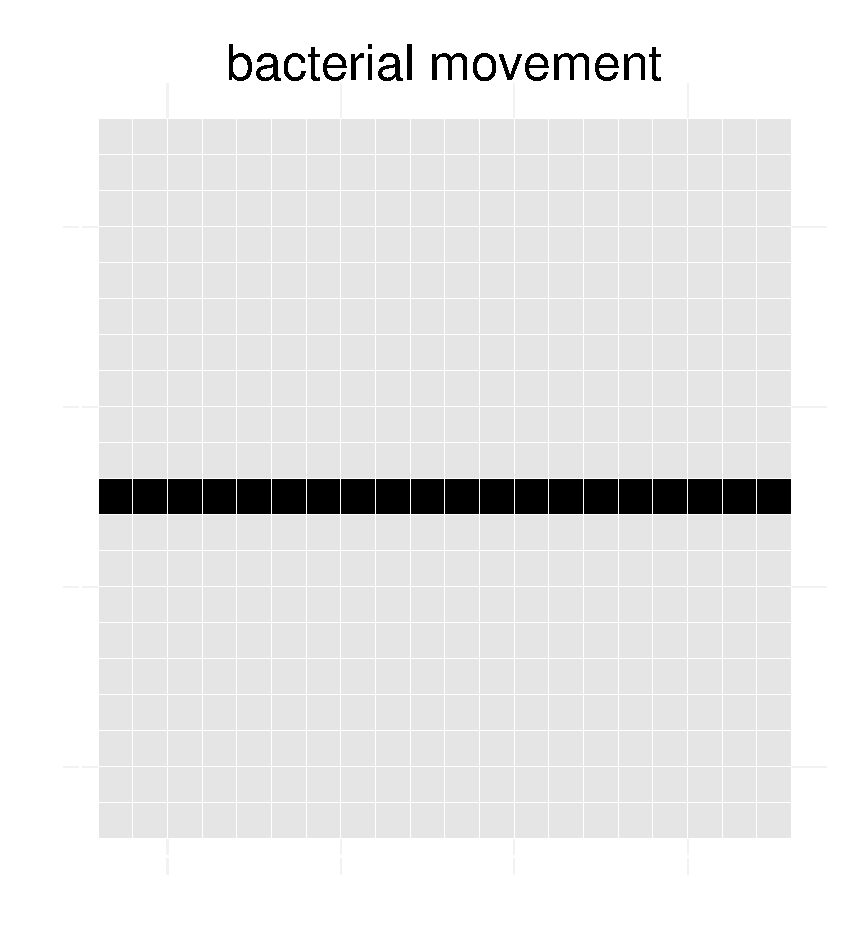
\includegraphics[width=\textwidth]{mov1.pdf}
  \end{minipage}
  \begin{minipage}[t]{0.3\textwidth}
    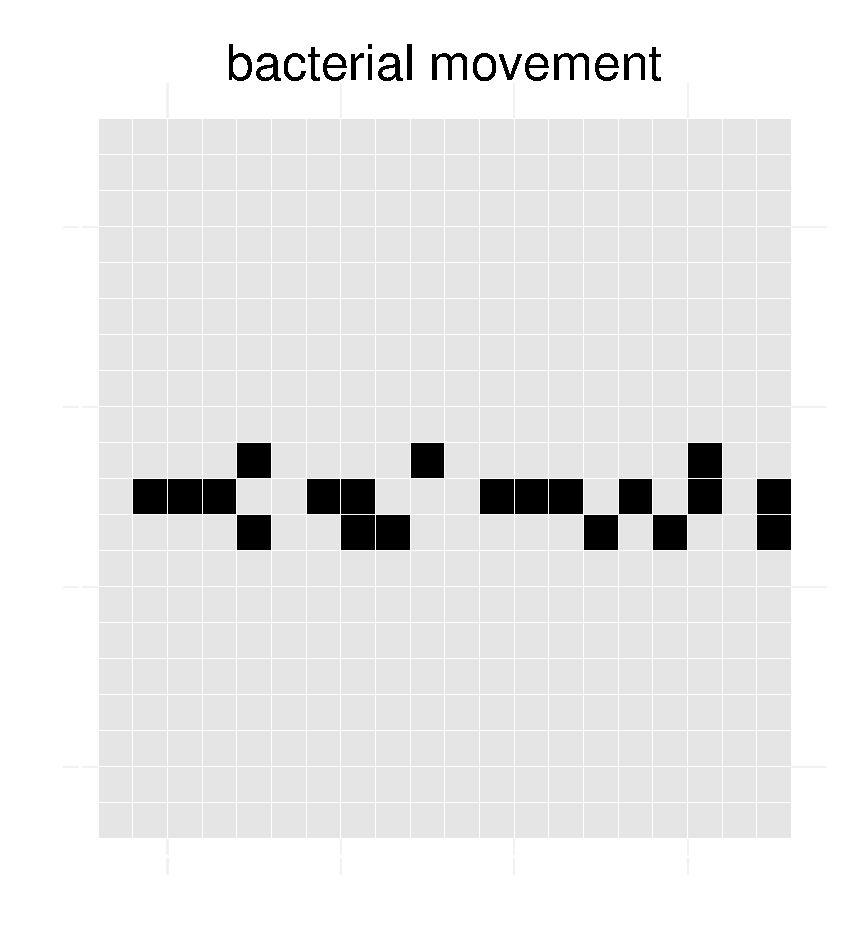
\includegraphics[width=\textwidth]{mov2.pdf}
  \end{minipage}
  \begin{minipage}[t]{0.3\textwidth}
    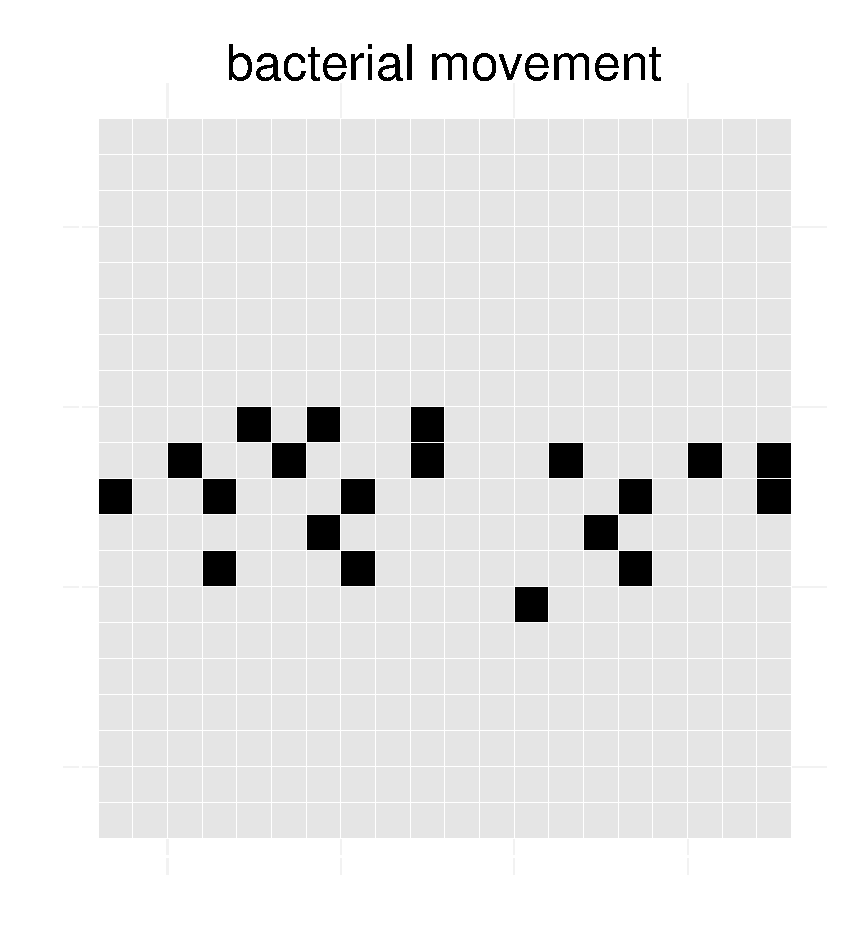
\includegraphics[width=\textwidth]{mov3.pdf}
  \end{minipage}
  \caption{Bacterial movement starting with a line of bacteria in the middle of a $20\times20$ grid. Three different iteration steps are displayed (time step 1, 2 and 5).}
  \label{fig:mov}
\end{figure}
\begin{figure}[h!]
  \centering
  \begin{minipage}[t]{0.3\textwidth}
    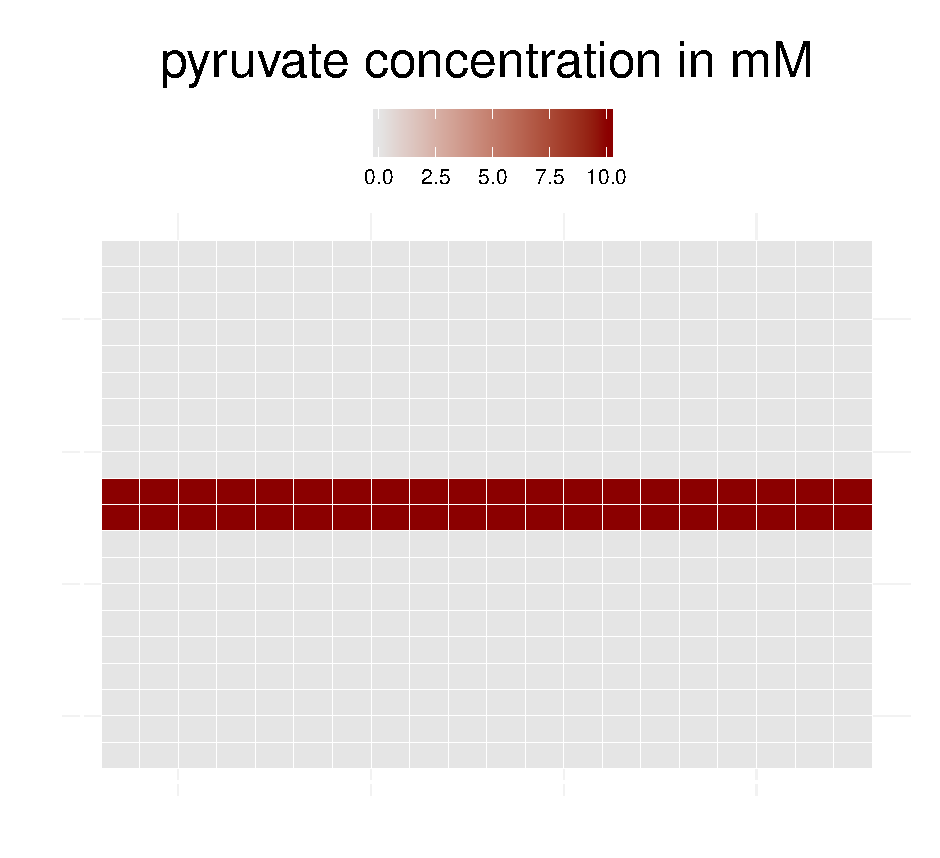
\includegraphics[width=\textwidth]{diff1.pdf}
  \end{minipage}
  \begin{minipage}[t]{0.3\textwidth}
    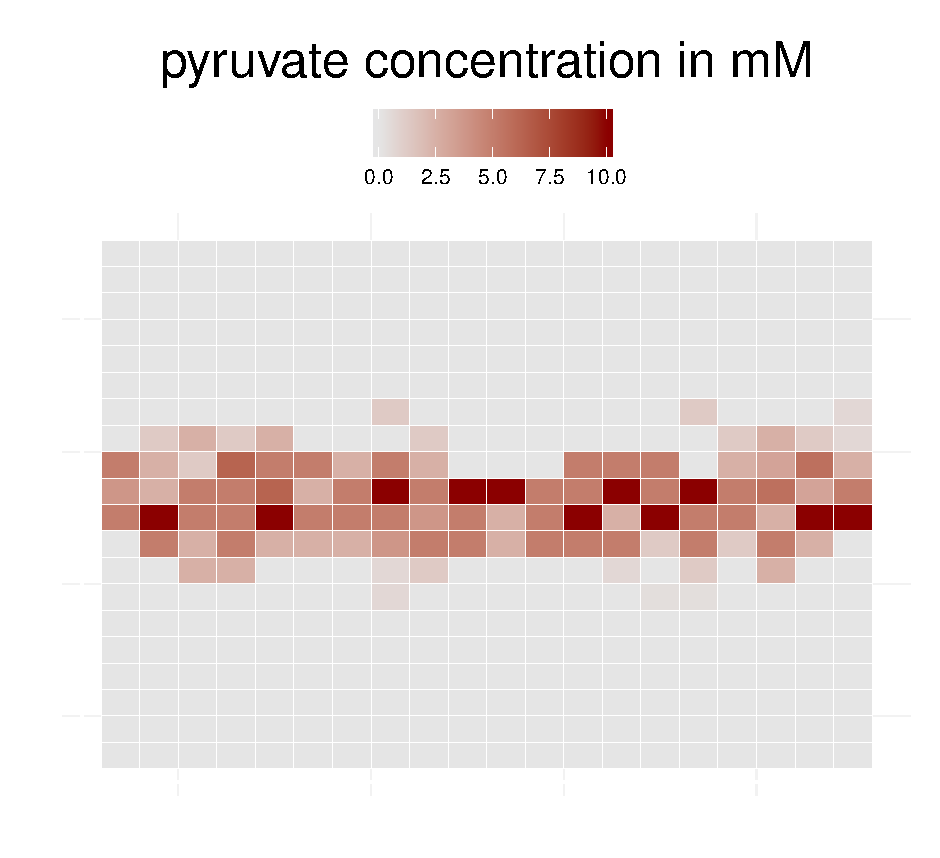
\includegraphics[width=\textwidth]{diff2.pdf}
  \end{minipage}
  \begin{minipage}[t]{0.3\textwidth}
    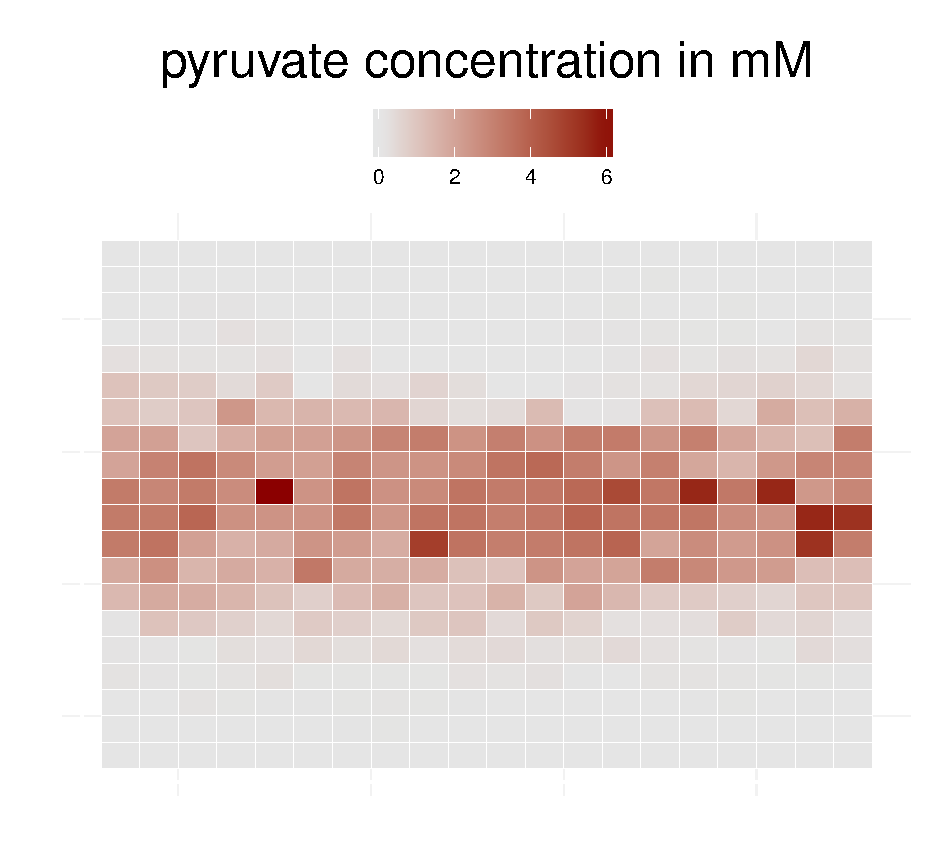
\includegraphics[width=\textwidth]{diff5.pdf}
  \end{minipage}
  \caption{Diffusion starting with 10\;mmol pyruvate in the middle of a $20\times20$ grid. Three different iteration steps are displayed (time step 1, 2 and 5).}
  \label{fig:diff}
\end{figure}

\subsubsection{Time consumption}

\begin{figure}[h!]
  \centering
  \subfigure[]{
  \begin{minipage}[t]{0.45\textwidth}
    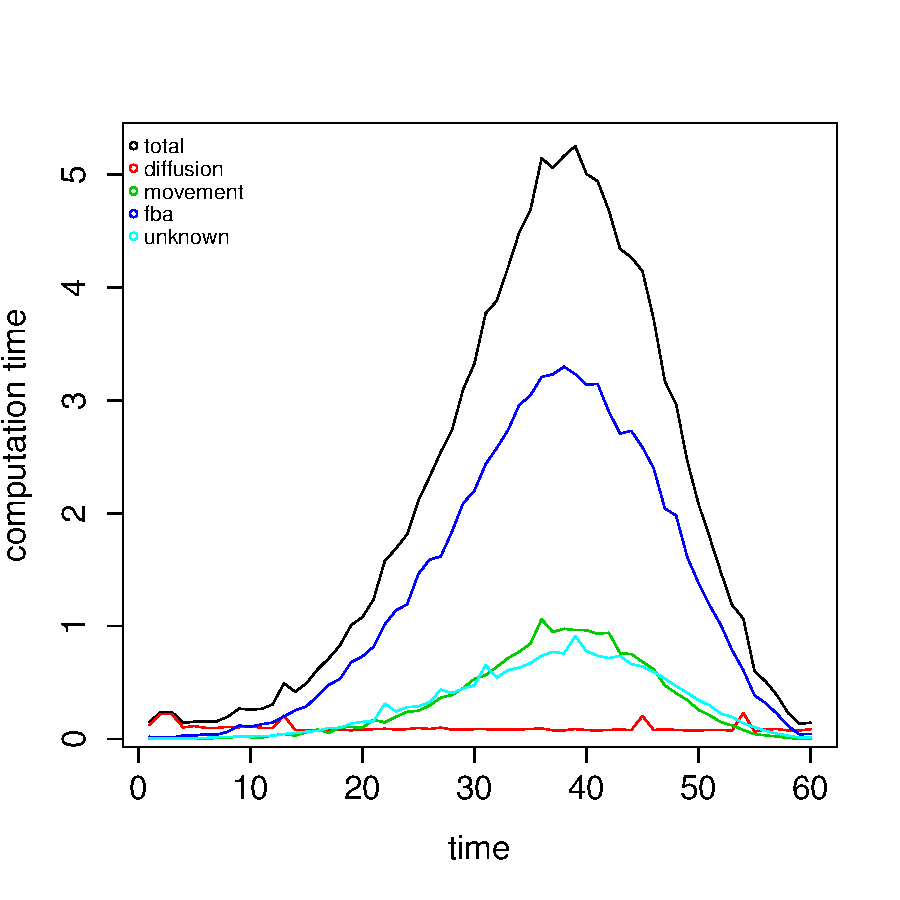
\includegraphics[width=\textwidth]{../results/img/ecoli_20x20_aerob_seed55_time_abs.pdf}
  \end{minipage}
  }
  \subfigure[]{
  \begin{minipage}[t]{0.45\textwidth}
    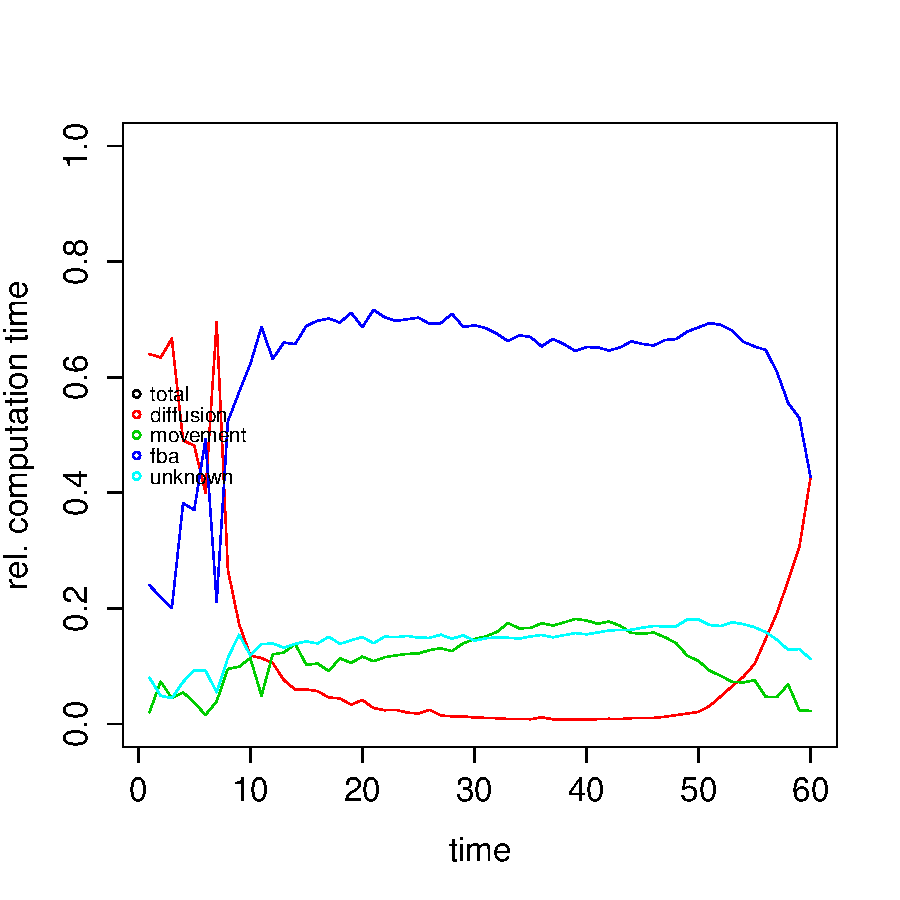
\includegraphics[width=\textwidth]{../results/img/ecoli_20x20_aerob_seed55_time_rel.pdf}
  \end{minipage}
  }
  \caption{Absolute (A) and relative (B) time consumption over the simulation of the \emph{E. coli} core model on a $20 \times 20$ grid.}
  \label{fig:time}
\end{figure}

Considering the time consumption of the whole framework (Figure \hyperref[fig:time]{\ref{fig:time}}), the calculation of the flux balance analysis required the highest amount of time.
Furthermore, the overall fba calculation time was dependent on the number of microbe individuals on the grid, whereat higher numbers of agents resulted in higher overall calculation times. The same was true for the movement function, which consumed after the fba the highest amount of time. The time consumption of diffusion function was considerably lower than the other functions and constant over the whole simulation, since it is independent on the number of microbes on the grid. Other
calculations for diverse matrix operations (primary $x$apply code in \textit{R}) required with respect to the movement a comparable small amount of time, but is significant, too.\\
Grid size was the dominant factor, because bigger space increased the needed time of all other parts: More diffusion, more bacteria, more movement, more fba.
For larger \textit{SBML} models the fba calculations consumed more time.
That's why the amount of metabolic reactions is only relevant for fba calculations.
The time consumption of the other function was independent on the used model and relativly insignificant for \textit{SBML} models taller than $500\times 500$ (reactions $\times$ metabolites).
Therefore, fba was the time limiting factor of the simulations.

\subsection{Population models}

\subsubsection{\textit{Escherichia coli} core}
The \textit{E. coli} core model was subjected to initial concentrations of the substrates glucose and oxygen to generate a population model and monitor the production/consumption of various metabolites (Figure \hyperref[fig:ecoresg]{\ref{fig:ecoresg}}). In the first time steps oxygen and glucose were consumed and CO$_2$ was produced. Additionally, fermentation products such as acetate, formate and ethanol were produced, which increased in concentration during the exponential phase of microbial growth. 
Acetate and formate were produced on high levels (averaged grid cell concentration of $> 60\, mmol$).
That's even more than CO$_2$ ($\approx 50\, mmol$).
The doubling time in the exponential phase was estimated as 7 iteration (h).
The population growth reached the stationary phase after 30 iterations (h), after all substrates were consumed. In the subsequent death phase no metabolites were produced or consumed.
According the dispersion of the microbes on the grid environment, substrates were consumed and metabolites produced (Figure \hyperref[fig:ecoregrids]{\ref{fig:ecoregrids}}).
\begin{figure}[h!]
  \centering
  \subfigure[]{
  %\begin{minipage}[t]{0.45\textwidth}
    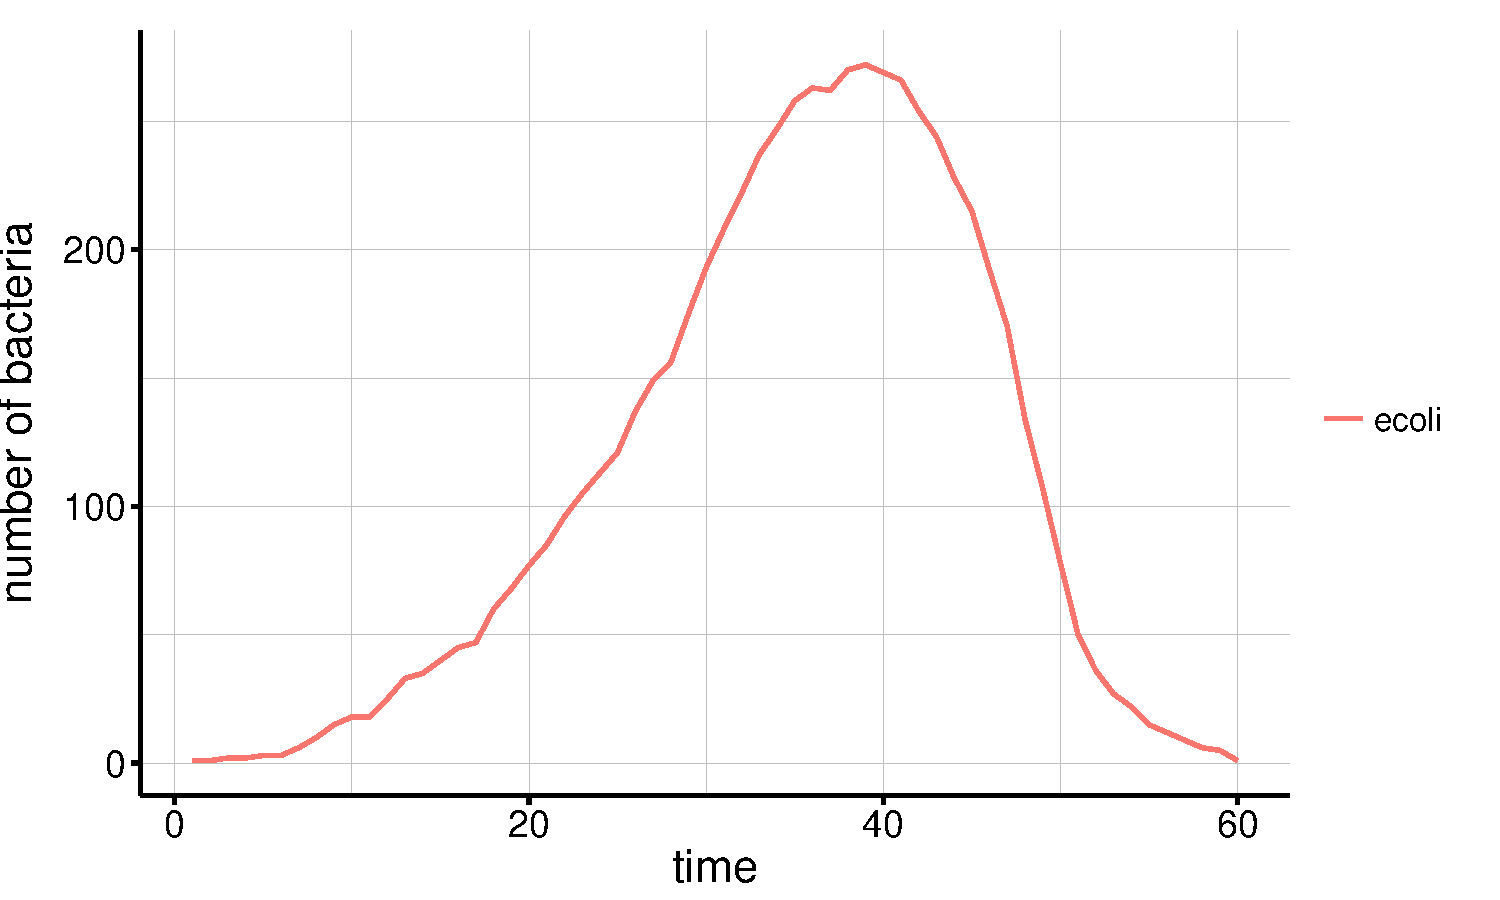
\includegraphics[scale=0.4]{../results/img/ecoli_20x20_aerob_seed55_growth.pdf}
  %\end{minipage}
  }
  \subfigure[]{
  %\begin{minipage}[t]{0.45\textwidth}
    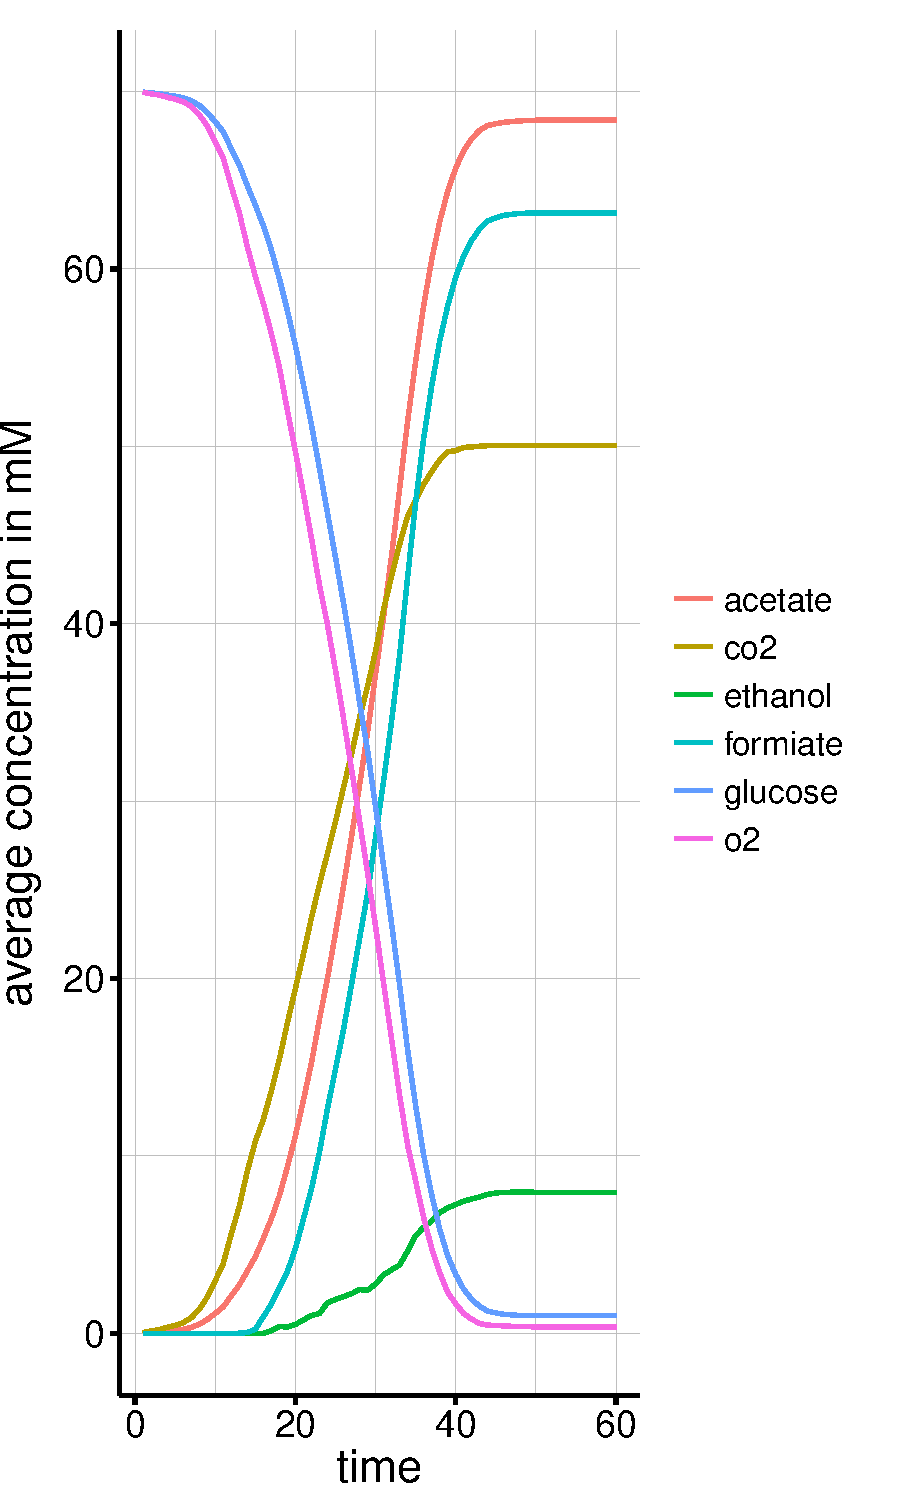
\includegraphics[scale=0.4]{../results/img/ecoli_20x20_aerob_seed55_subs.pdf}
  %\end{minipage}
  }
  \caption{Population dynamics of the \emph{E. coli} core model on a $20\times20$ grid, with bacterial growth (A) and consumption/production of various metabolites (B). An initial concentration of 70\;mmol per grid cell of glucose and oxygen was added to the environment. The seed of the random number generator was set to 55.}
\label{fig:ecoresg}
\end{figure}
\begin{figure}[h!]
  \centering
  \subfigure[]{
    \begin{minipage}[t]{0.3\textwidth}
    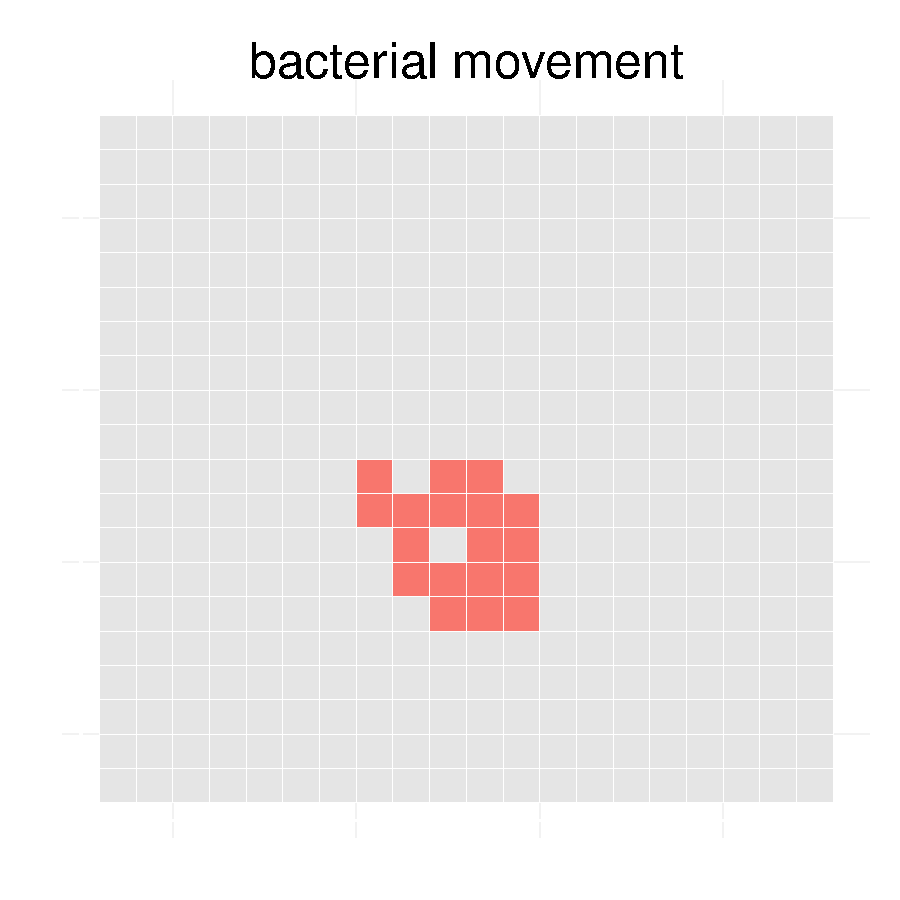
\includegraphics[width=\textwidth]{../results/img/ecoli_20x20_aerob_seed55_bac10.pdf}
  \end{minipage}
  \begin{minipage}[t]{0.3\textwidth}
    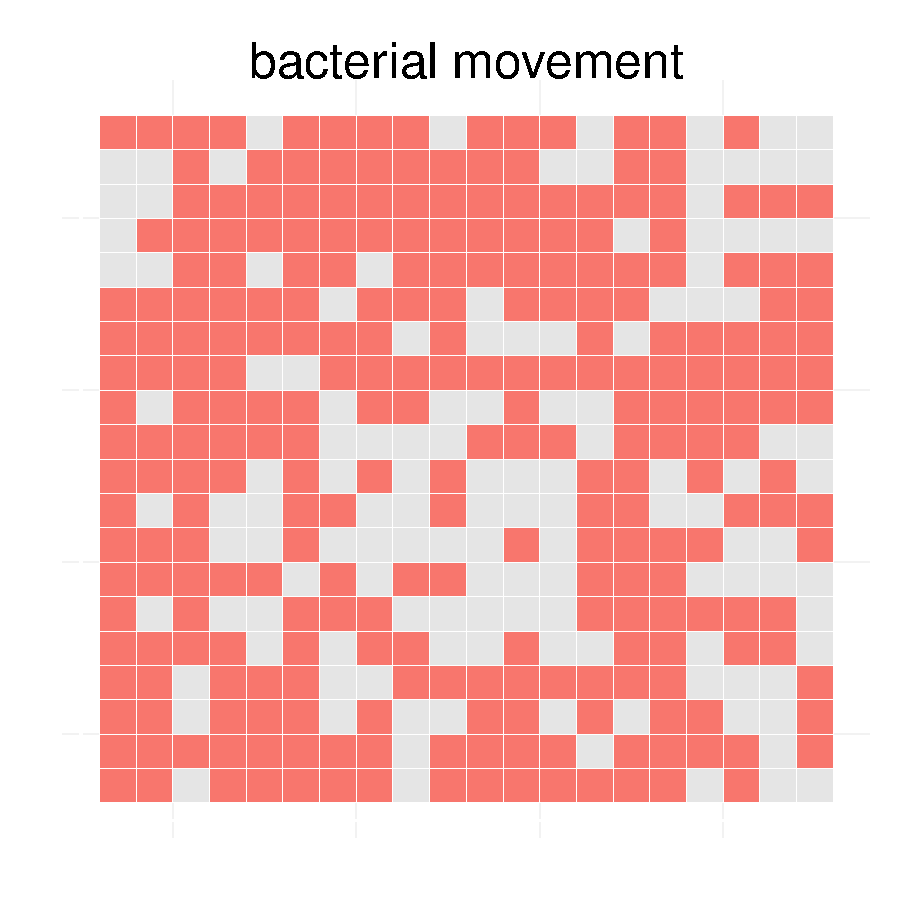
\includegraphics[width=\textwidth]{../results/img/ecoli_20x20_aerob_seed55_bac40.pdf}
  \end{minipage}
  \begin{minipage}[t]{0.3\textwidth}
    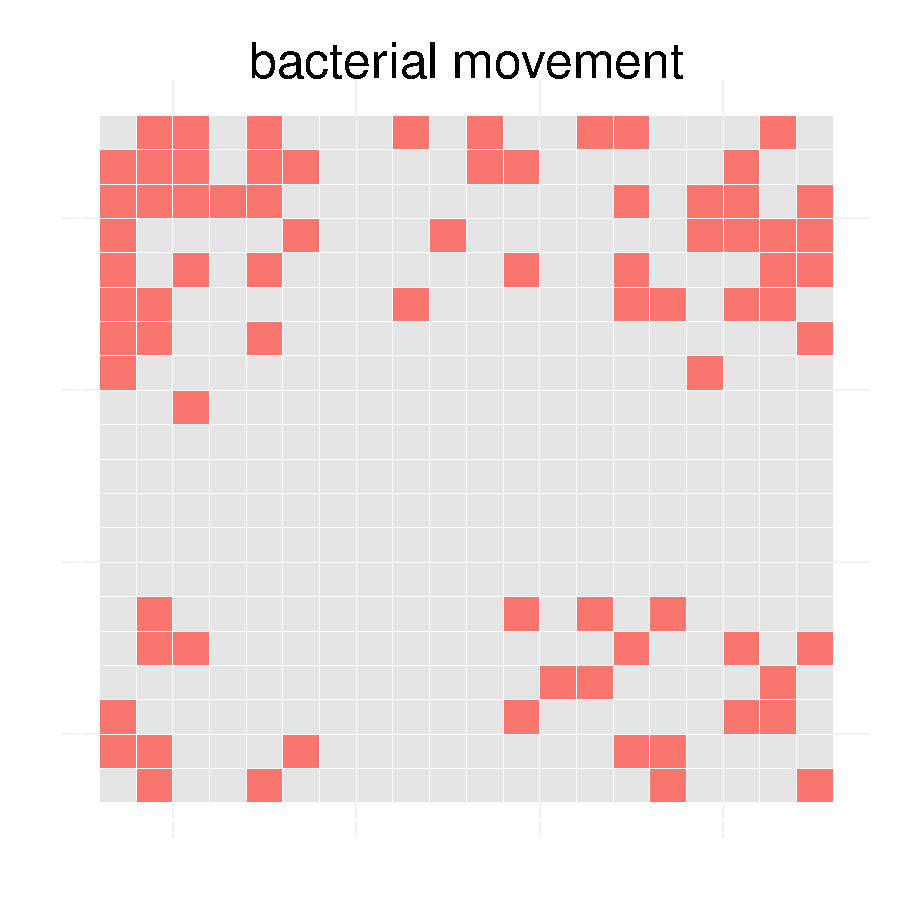
\includegraphics[width=\textwidth]{../results/img/ecoli_20x20_aerob_seed55_bac50.pdf}
  \end{minipage}
  }
  \subfigure[]{
  \begin{minipage}[t]{0.3\textwidth}
    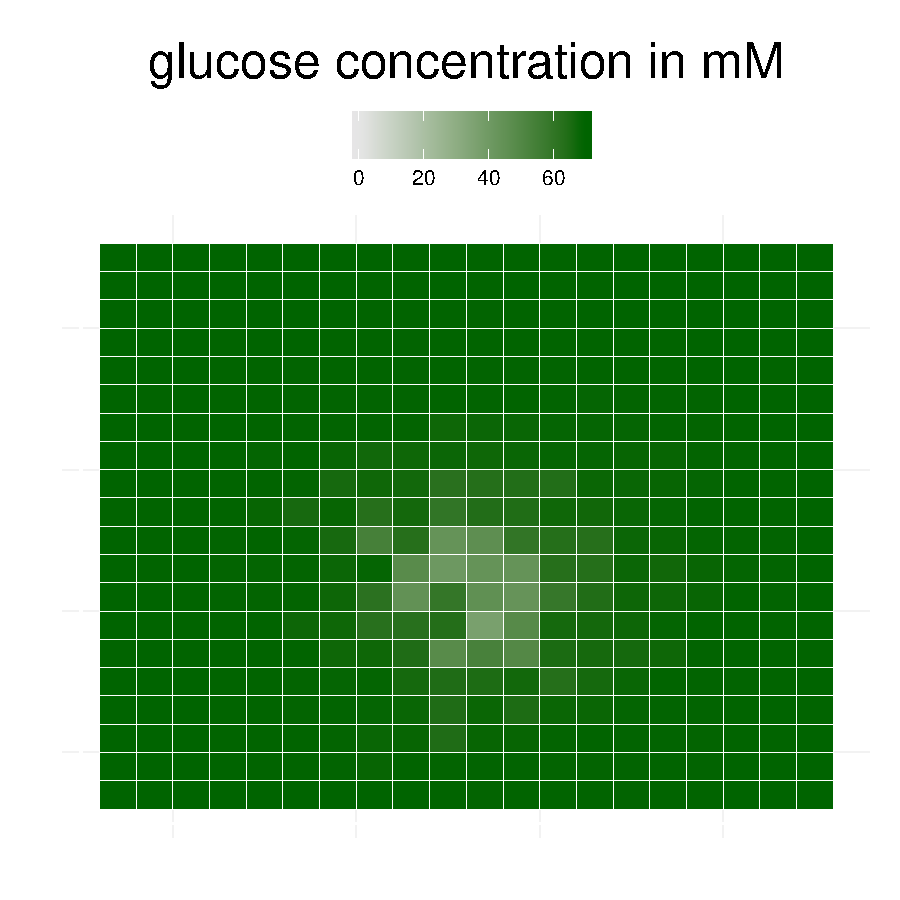
\includegraphics[width=\textwidth]{../results/img/ecoli_20x20_aerob_seed55_glc10.pdf}
  \end{minipage}
  \begin{minipage}[t]{0.3\textwidth}
    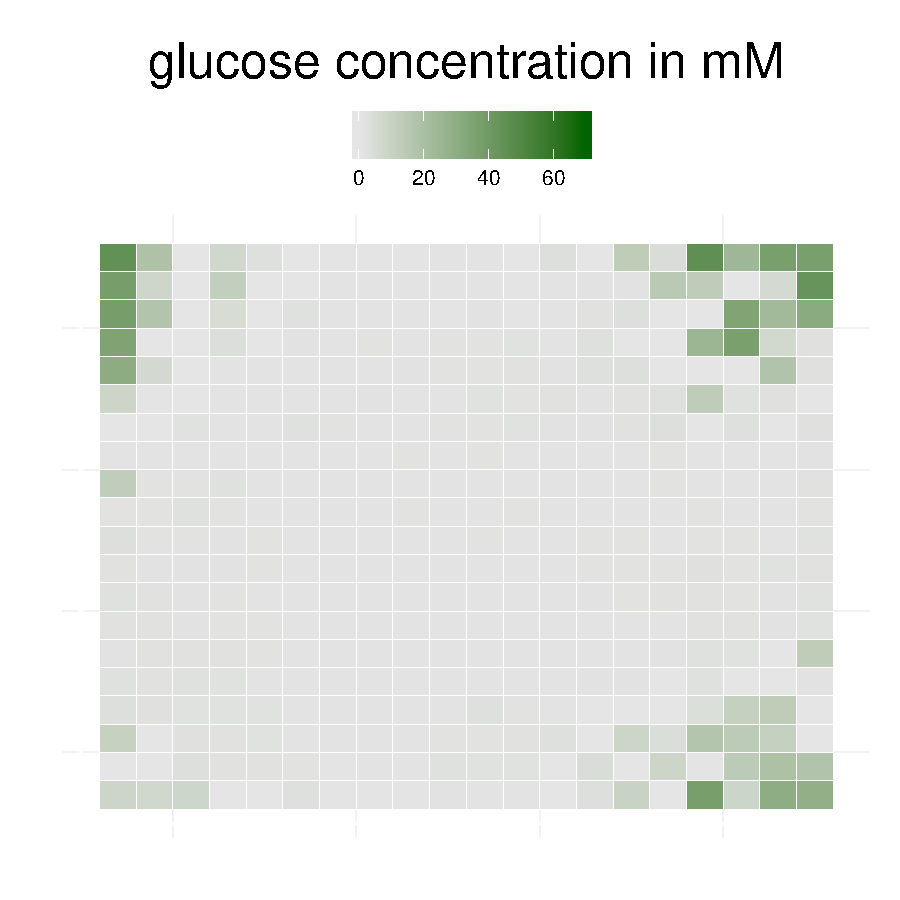
\includegraphics[width=\textwidth]{../results/img/ecoli_20x20_aerob_seed55_glc40.pdf}
  \end{minipage}
  \begin{minipage}[t]{0.3\textwidth}
    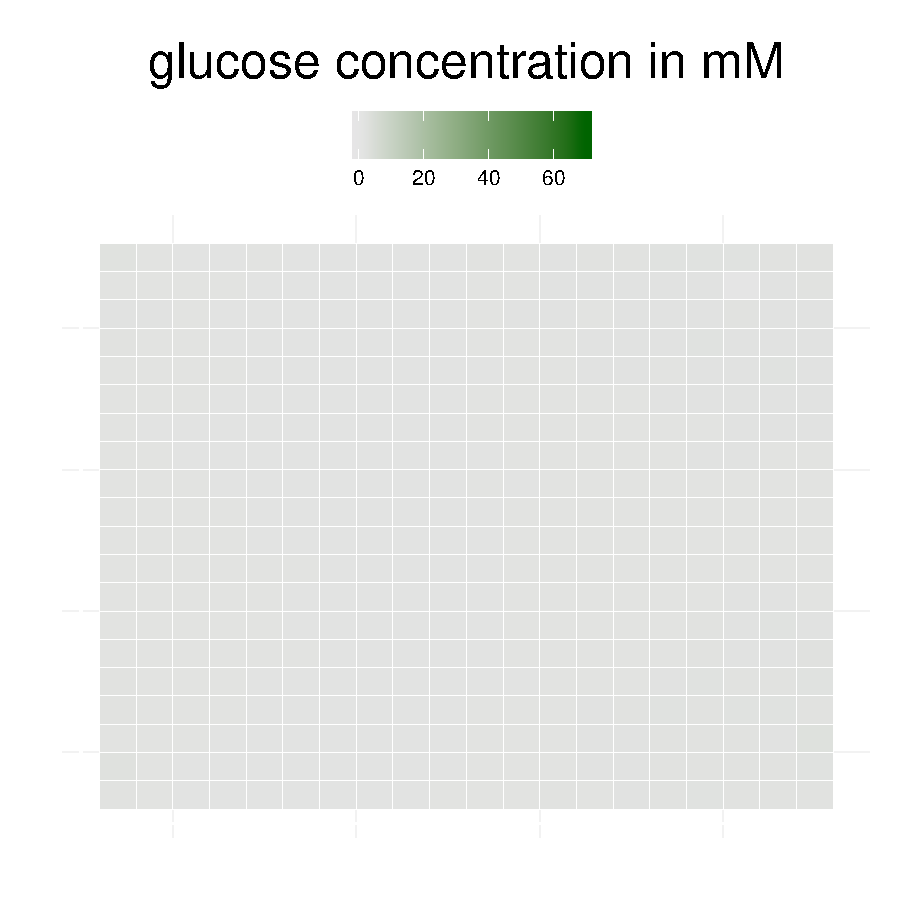
\includegraphics[width=\textwidth]{../results/img/ecoli_20x20_aerob_seed55_glc50.pdf}
  \end{minipage}
  }
  \subfigure[]{
  \begin{minipage}[t]{0.3\textwidth}
    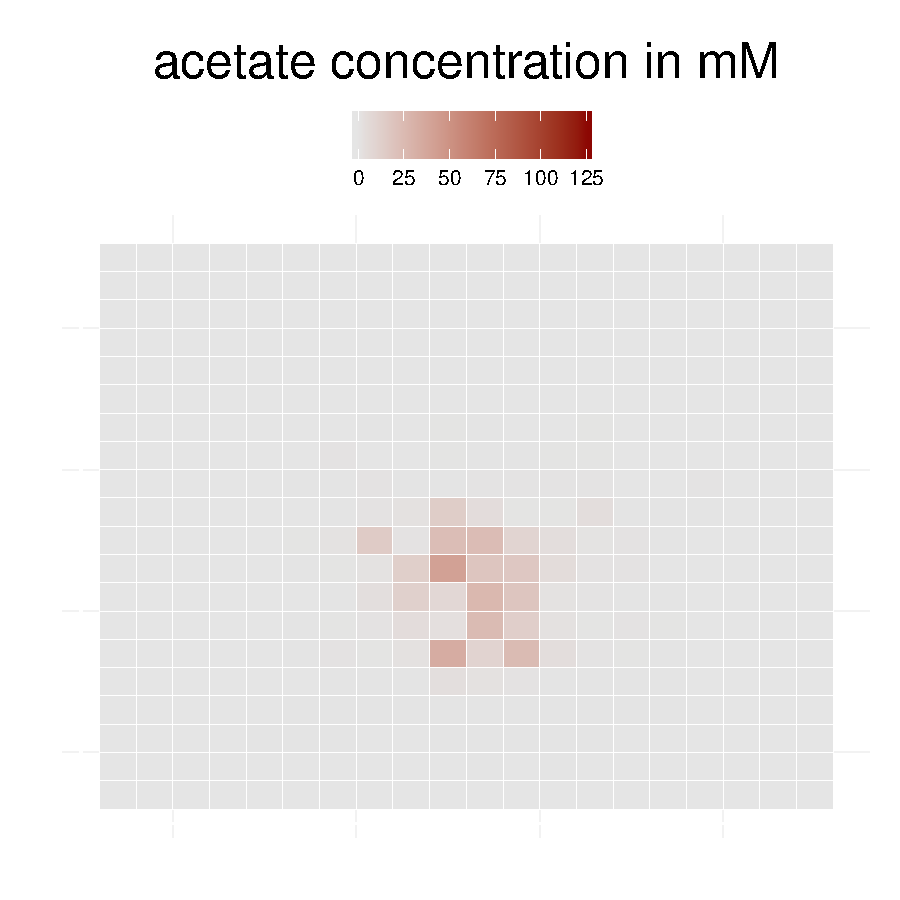
\includegraphics[width=\textwidth]{../results/img/ecoli_20x20_aerob_seed55_ace10.pdf}
  \end{minipage}
  \begin{minipage}[t]{0.3\textwidth}
    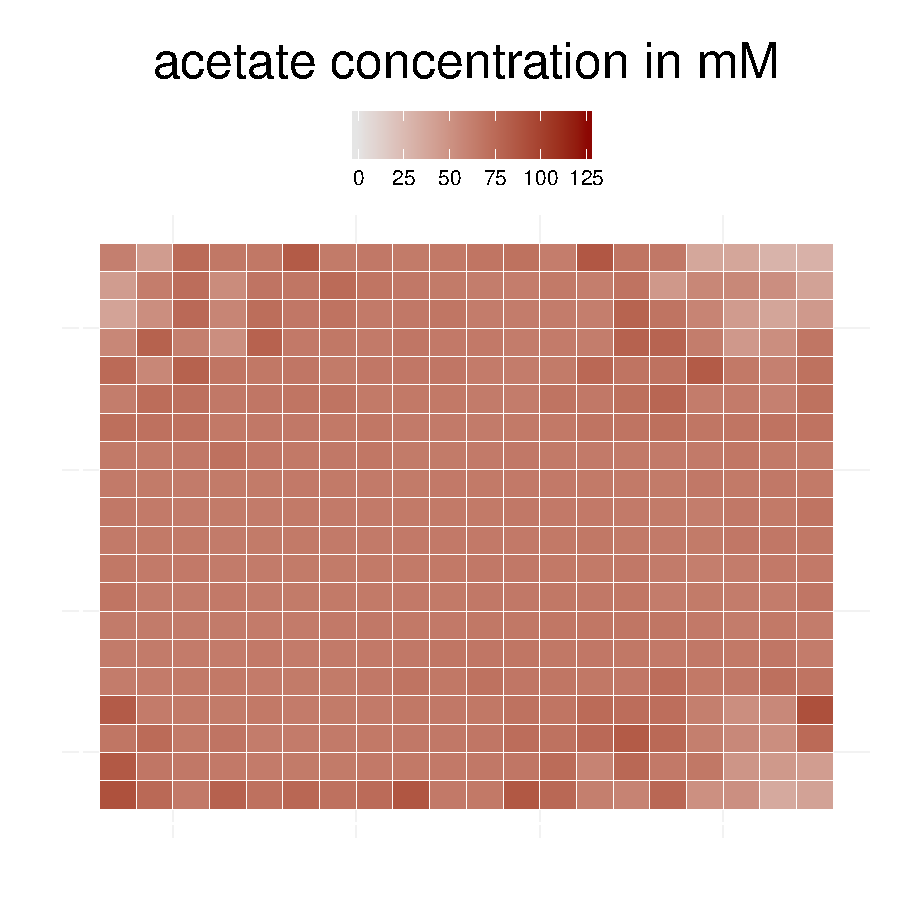
\includegraphics[width=\textwidth]{../results/img/ecoli_20x20_aerob_seed55_ace40.pdf}
  \end{minipage}
  \begin{minipage}[t]{0.3\textwidth}
    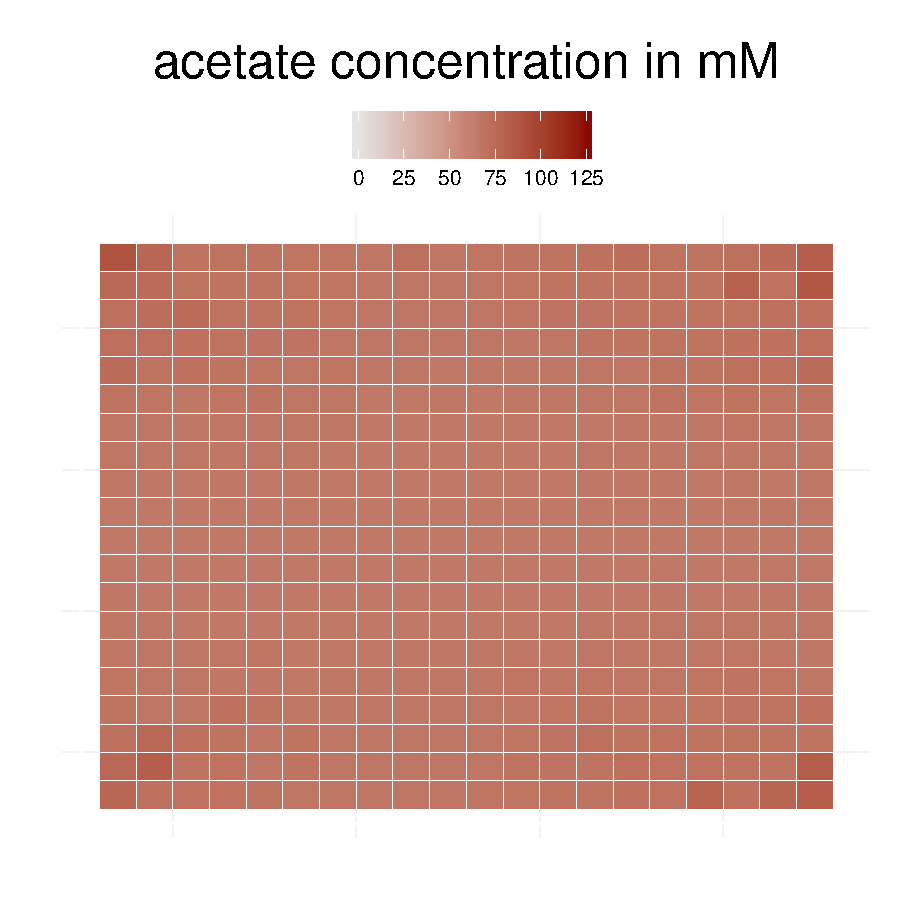
\includegraphics[width=\textwidth]{../results/img/ecoli_20x20_aerob_seed55_ace50.pdf}
  \end{minipage}
  }
  \subfigure[]{
  \begin{minipage}[t]{0.3\textwidth}
    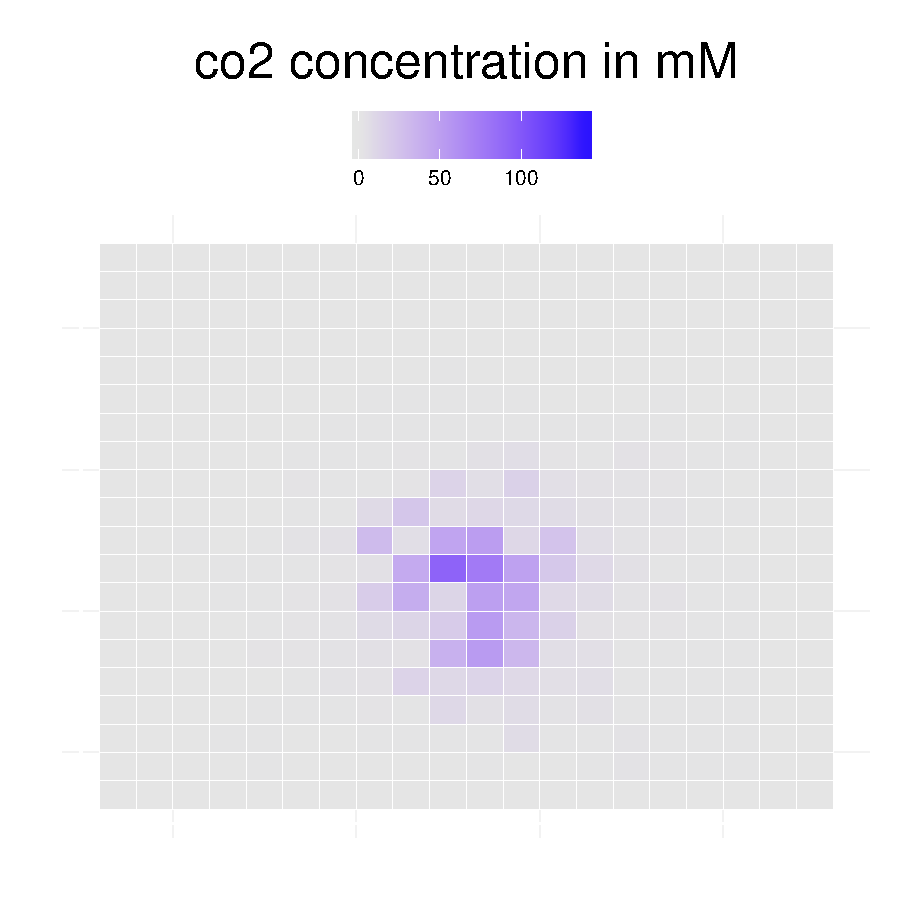
\includegraphics[width=\textwidth]{../results/img/ecoli_20x20_aerob_seed55_co210.pdf}
  \end{minipage}
  \begin{minipage}[t]{0.3\textwidth}
    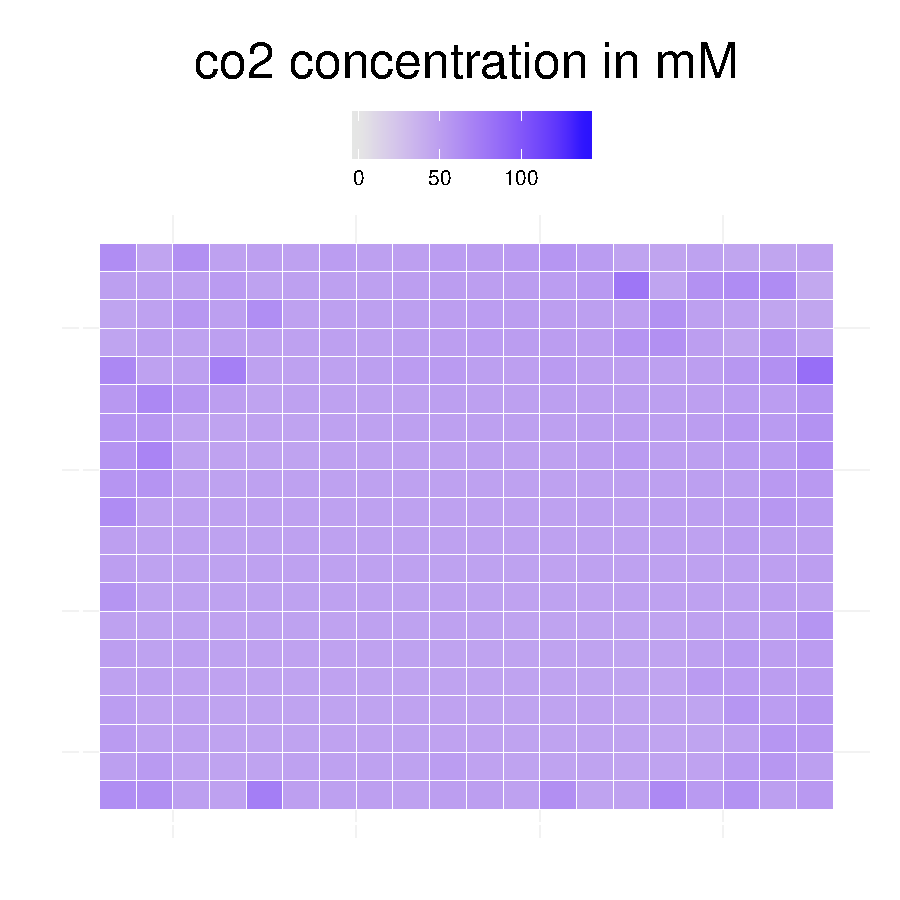
\includegraphics[width=\textwidth]{../results/img/ecoli_20x20_aerob_seed55_co240.pdf}
  \end{minipage}
  \begin{minipage}[t]{0.3\textwidth}
    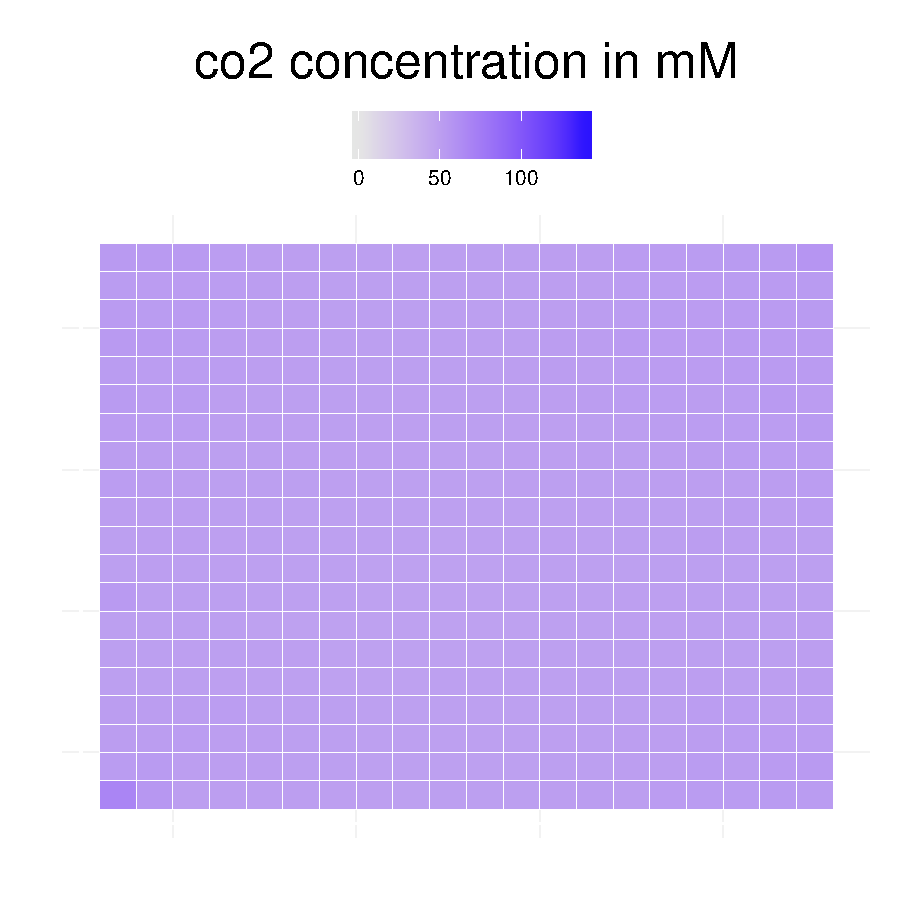
\includegraphics[width=\textwidth]{../results/img/ecoli_20x20_aerob_seed55_co250.pdf}
  \end{minipage}
  }
  %\caption{Population and metabolite dynamics of the \emph{E. coli} core model on a $20\times20$ grid.}
  \caption{Population dynamics of the \emph{E. coli} core model on a $20\times20$ grid, with bacterial movement (A) and concentrations of glucose (B), acetate (C) and CO$_2$ (D) (of time step 10, 40 and 50). The seed of the random number generator was set to 55.}
  \label{fig:ecoregrids}
\end{figure}

\subsubsection{\textit{Escherichia coli big (,,Bcoli'')}}
%\label{Bcoli}
%The \textit{E. coli} model was subjected to initial concentrations of the substrates glucose and oxygen to generate a population model and monitor the production/consumption of various metabolites (Figure \hyperref[fig:ecolisg]{\ref{fig:ecolisg}}). In the first time steps oxygen and glucose were consumed and CO$_2$ was produced. Additionally, few time steps later fermentation products such as acetate and ethanol were produced, which increased in concentration during the exponential phase of microbial growth. 
%CO$_2$ reached average grid cell concentration of $\approx 120\, mmol$, acetate $\approx 50\, mmol$ and ethanol had a final concentration of $\approx 10\,mmol$.
%In the simulation, no production of formate was found. The doubling time in the exponential phase was estimated as 6 iteration (h).
%
%The population growth reached the stationary phase in approximately 30 iterations (h), after all substrates were consumed. In the subsequent death phase no metabolites were produced or consumed. The population died out after 60 iterations.
%
%According the dispersion of the microbes on the grid environment, substrates were consumed and metabolites produced (Figure \hyperref[fig:ecoligrids]{\ref{fig:ecoligrids}}). Here, CO$_2$ was produced on every position the bacterial agents visited and  acetate was preferably produced in the centre of the grid.
%\begin{figure}[h!]
%  \centering
%    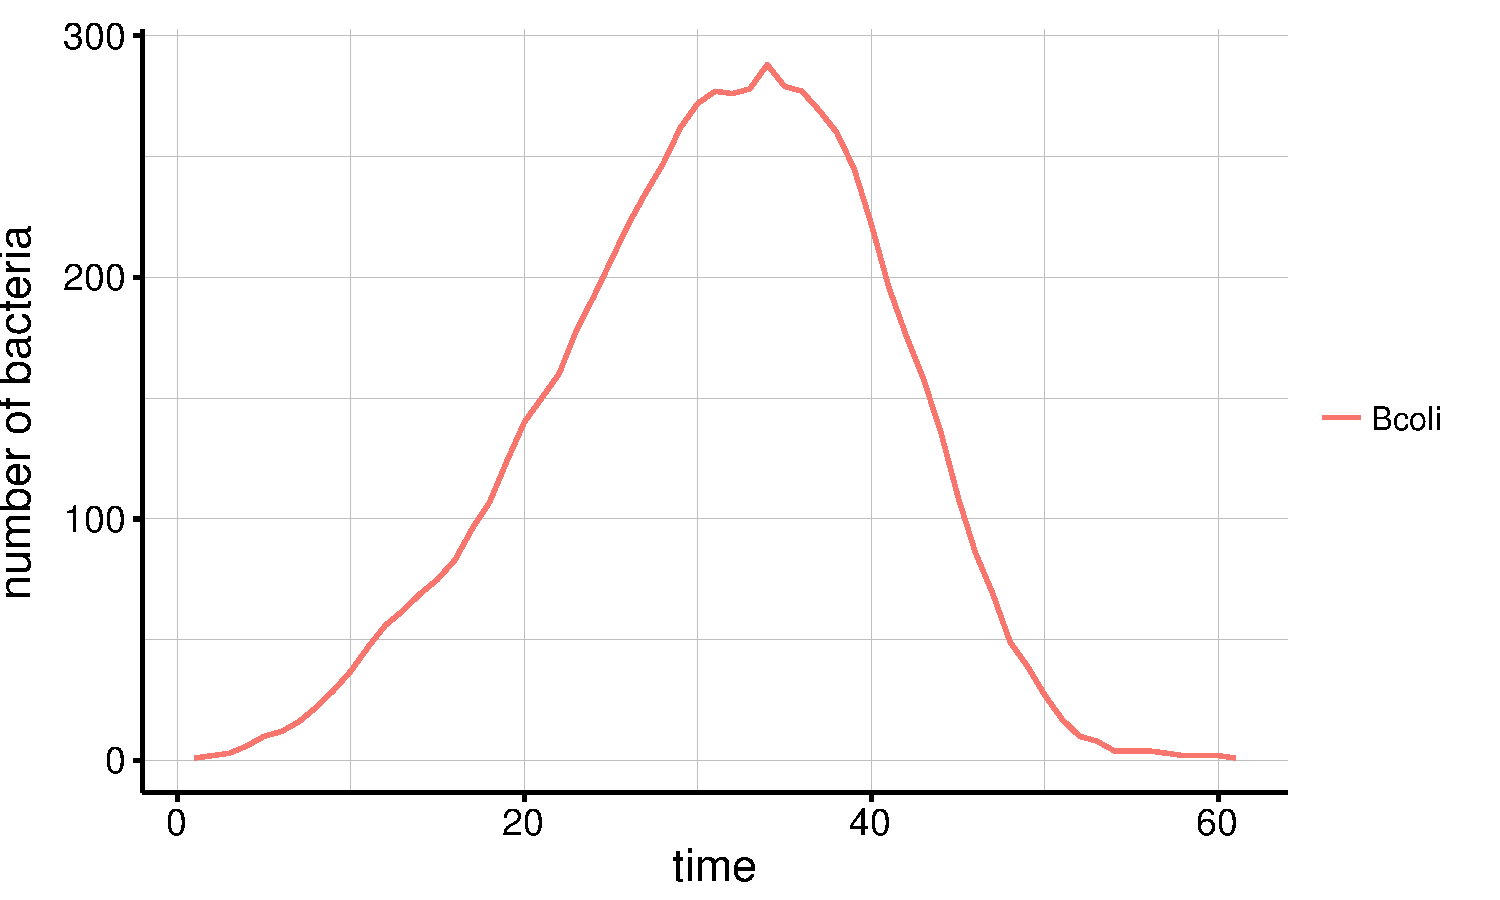
\includegraphics[scale=0.4]{../results/img/Bcoli_20x20_seed176_growth.pdf}
%    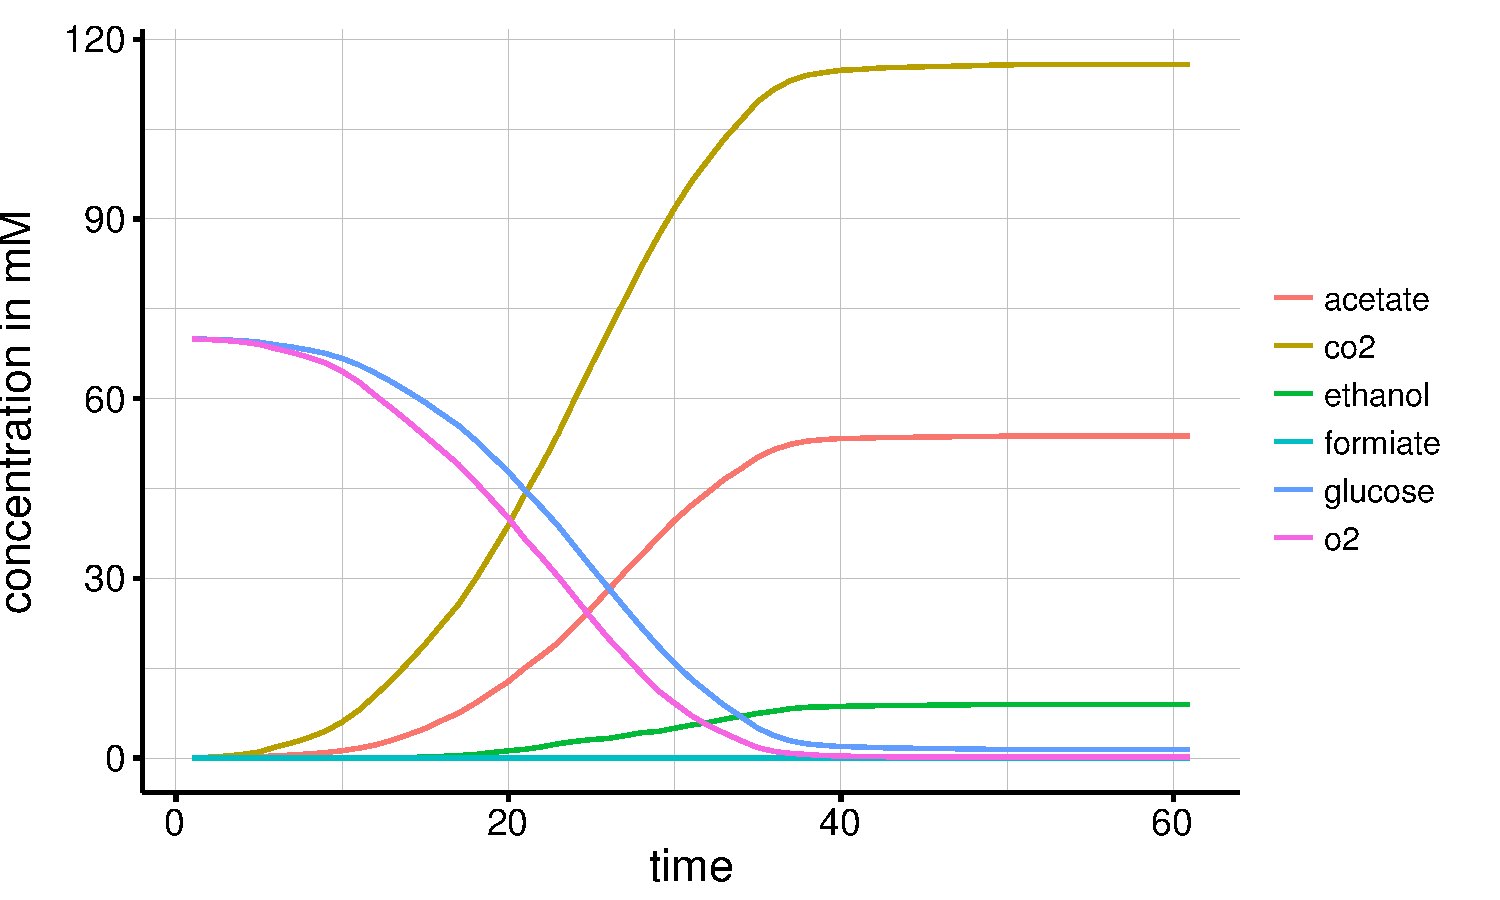
\includegraphics[scale=0.4]{../results/img/Bcoli_20x20_seed176_subs.pdf}
%  \caption{Population dynamics of the big \emph{E. coli} model on a $20\times20$ grid, with bacterial growth (A) and consumption/production of various metabolites (B). An initial concentration of 70\;mmol per grid cell of glucose and oxygen was added to the environment. The seed of the random number generator was set to 176.}
%  \label{fig:ecolisg}
%\end{figure}
%\begin{figure}[h!]
%  \centering
%  \subfigure[]{
%    \begin{minipage}[t]{0.3\textwidth}
%    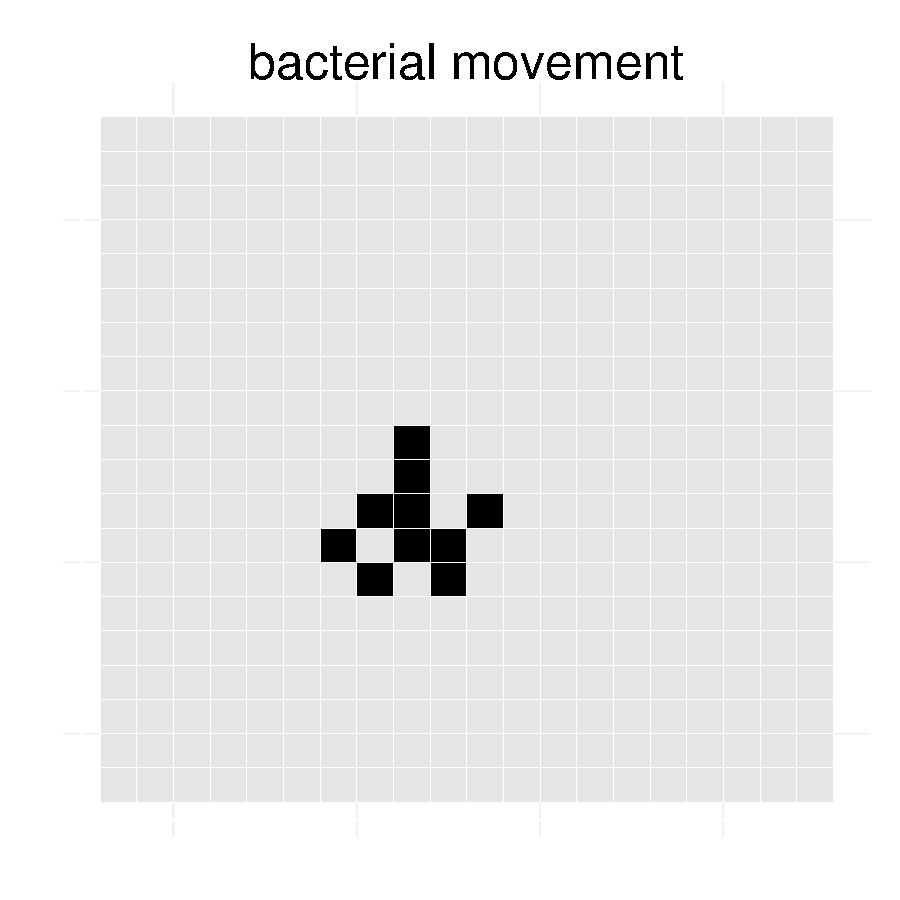
\includegraphics[width=\textwidth]{../results/img/Bcoli_20x20_seed176_bac5.pdf}
%  \end{minipage}
%  \begin{minipage}[t]{0.3\textwidth}
%    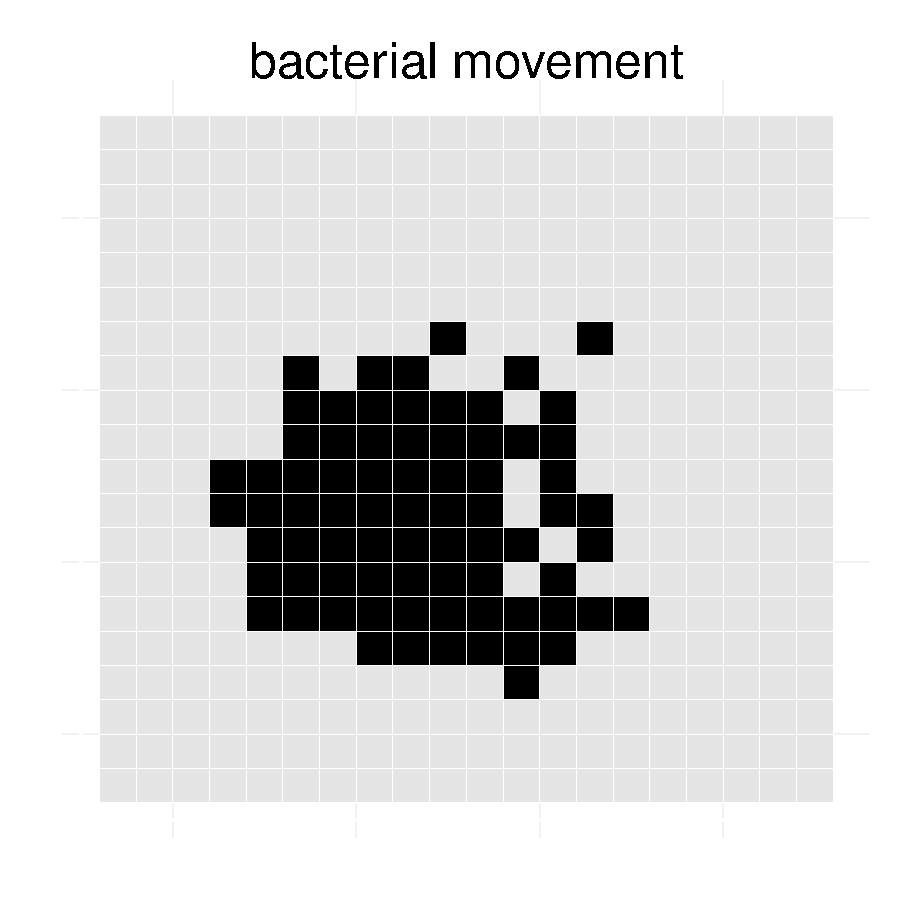
\includegraphics[width=\textwidth]{../results/img/Bcoli_20x20_seed176_bac15.pdf}
%  \end{minipage}
%  \begin{minipage}[t]{0.3\textwidth}
%    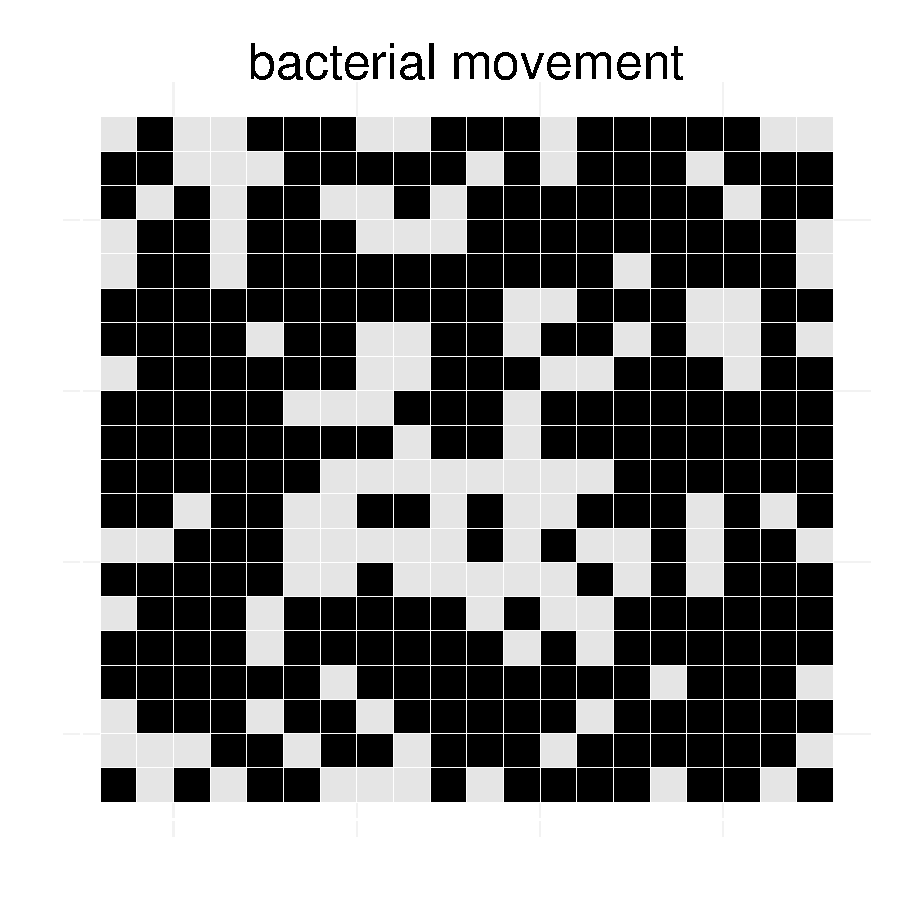
\includegraphics[width=\textwidth]{../results/img/Bcoli_20x20_seed176_bac35.pdf}
%  \end{minipage}
%  }
%  \subfigure[]{
%  \begin{minipage}[t]{0.3\textwidth}
%    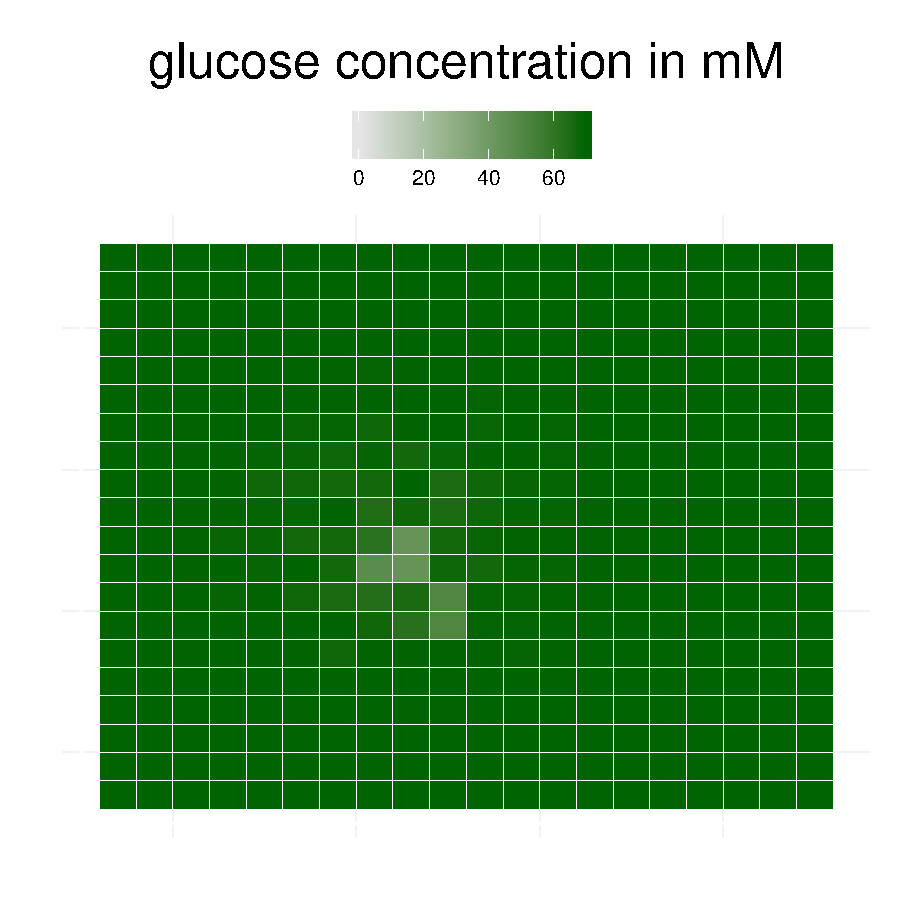
\includegraphics[width=\textwidth]{../results/img/Bcoli_20x20_seed176_glucose5a.pdf}
%  \end{minipage}
%  \begin{minipage}[t]{0.3\textwidth}
%    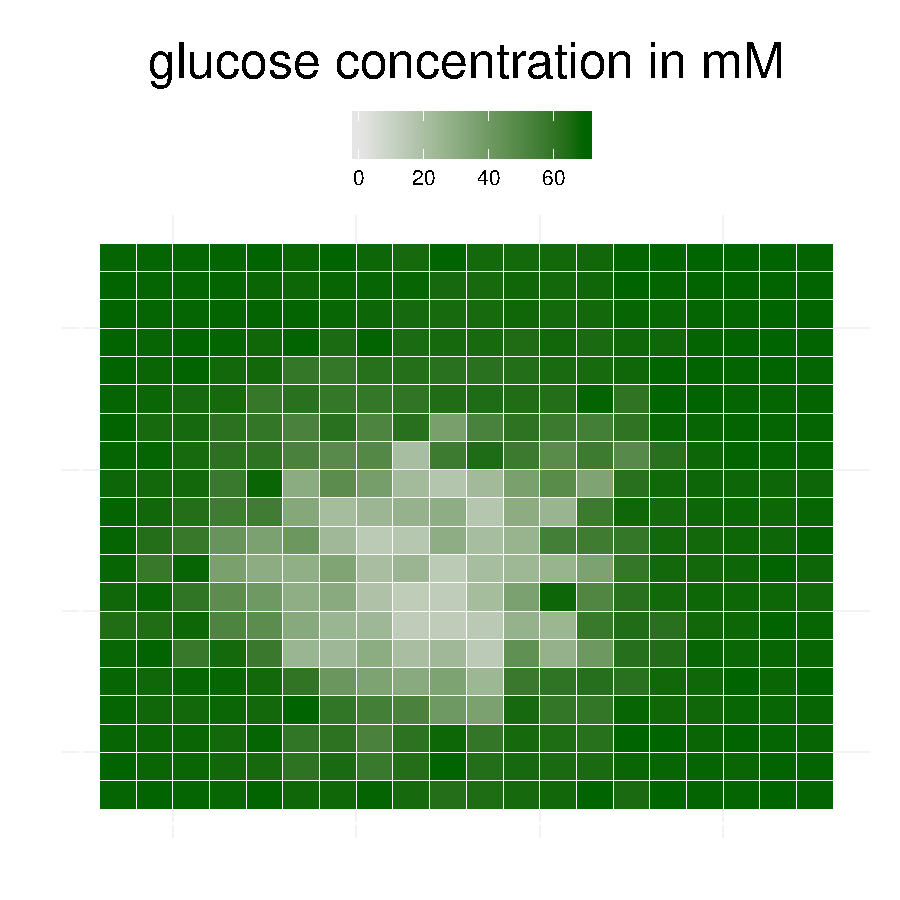
\includegraphics[width=\textwidth]{../results/img/Bcoli_20x20_seed176_glucose15.pdf}
%  \end{minipage}
%  \begin{minipage}[t]{0.3\textwidth}
%    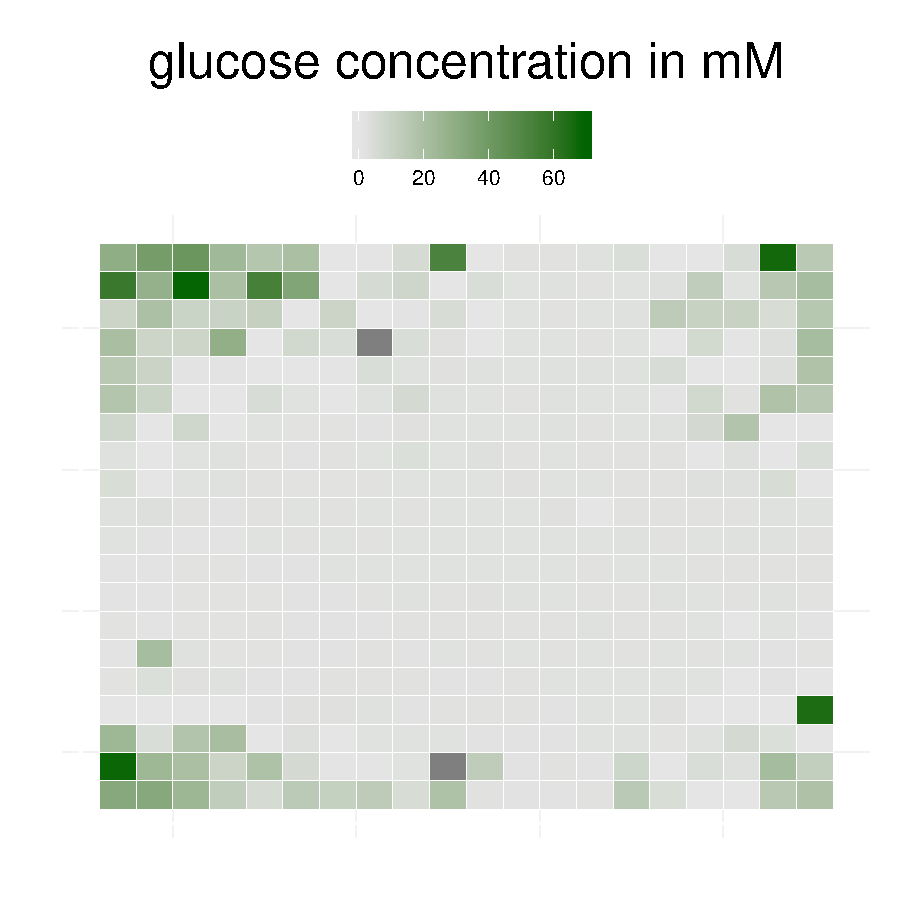
\includegraphics[width=\textwidth]{../results/img/Bcoli_20x20_seed176_glucose35a.pdf}
%  \end{minipage}
%  }
%  \subfigure[]{
%  \begin{minipage}[t]{0.3\textwidth}
%    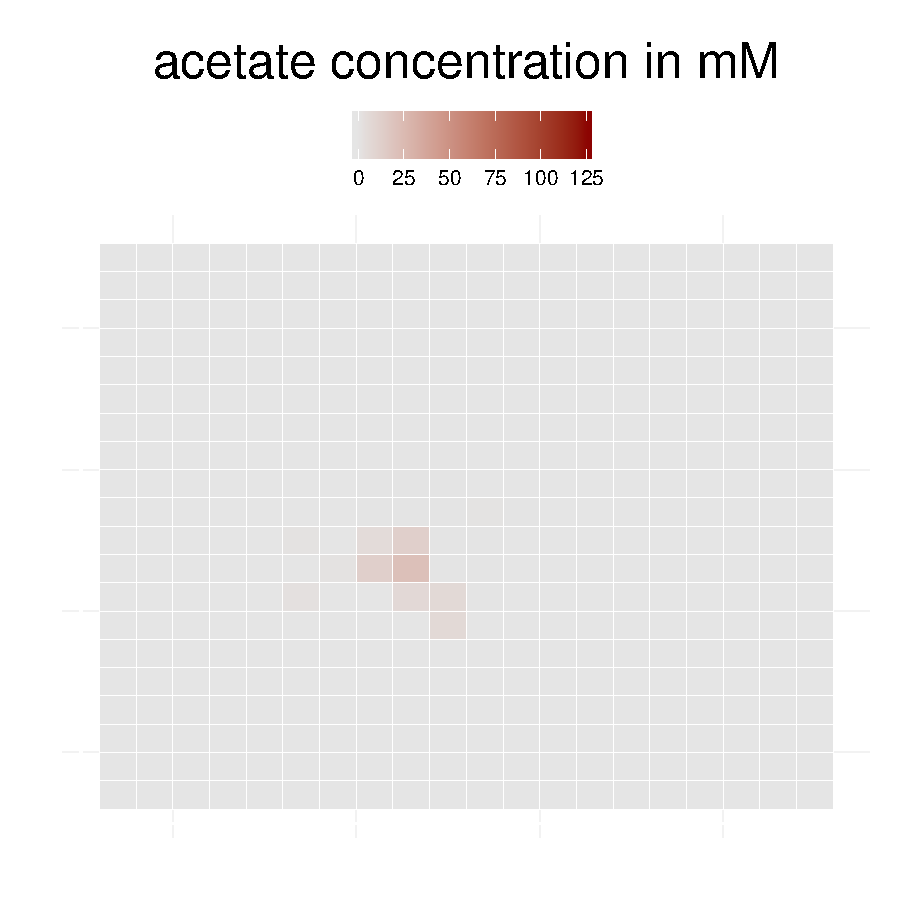
\includegraphics[width=\textwidth]{../results/img/Bcoli_20x20_seed176_ace5a.pdf}
%  \end{minipage}
%  \begin{minipage}[t]{0.3\textwidth}
%    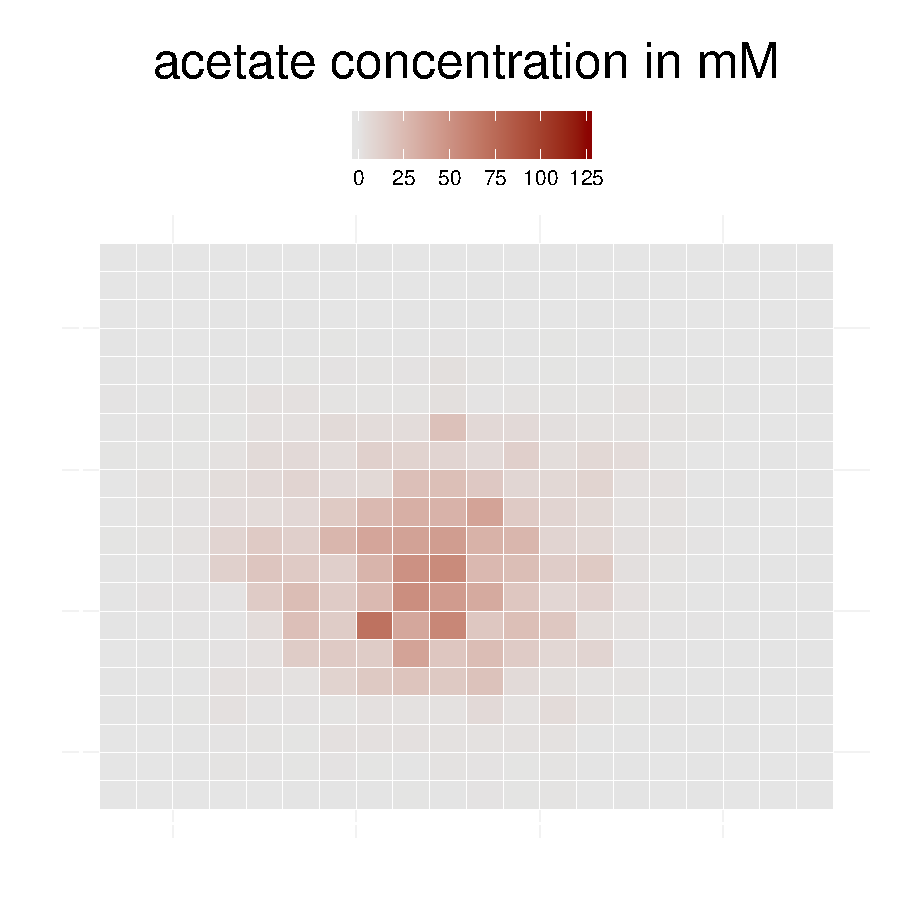
\includegraphics[width=\textwidth]{../results/img/Bcoli_20x20_seed176_ace15.pdf}
%  \end{minipage}
%  \begin{minipage}[t]{0.3\textwidth}
%    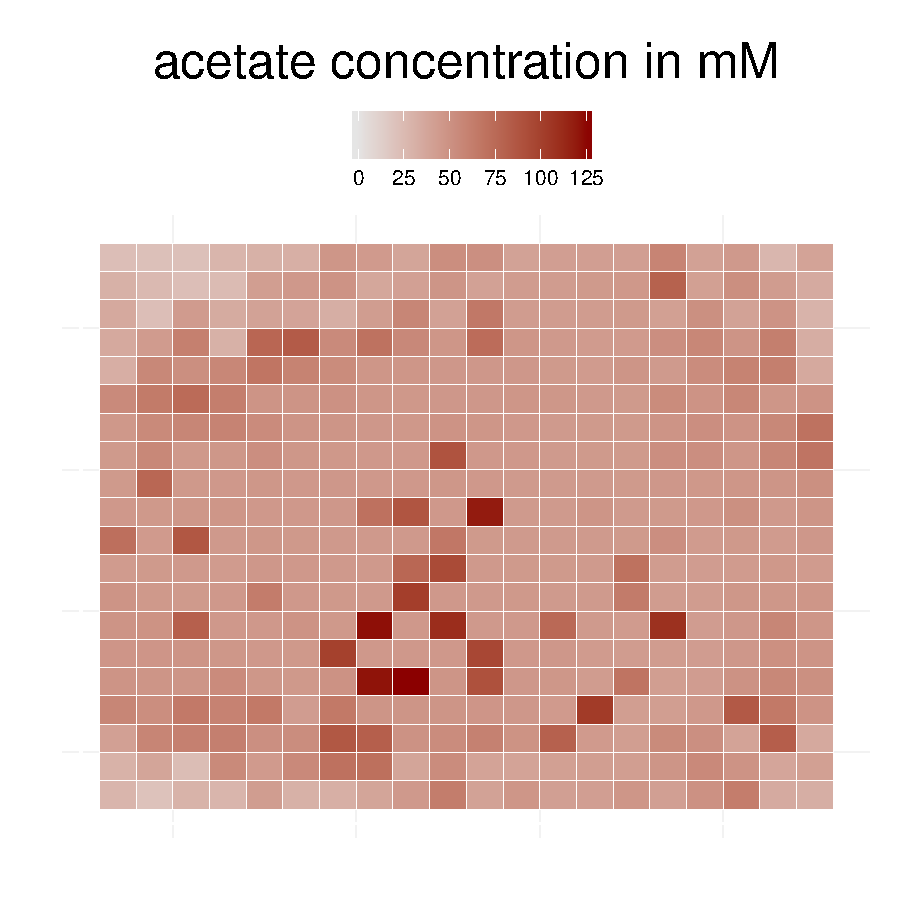
\includegraphics[width=\textwidth]{../results/img/Bcoli_20x20_seed176_ace35a.pdf}
%  \end{minipage}Figure \hyperref[fig:diff]{\ref{fig:diff}}
%  }
%  \subfigure[]{
%  \begin{minipage}[t]{0.3\textwidth}
%    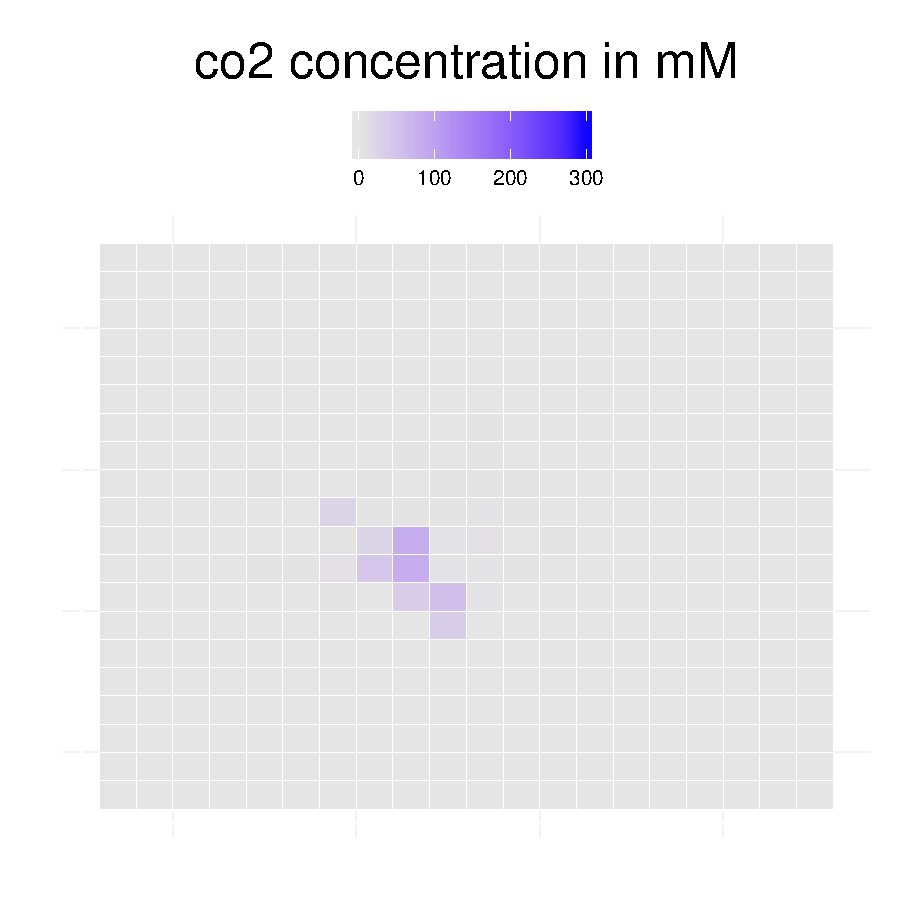
\includegraphics[width=\textwidth]{../results/img/Bcoli_20x20_seed176_co25a.pdf}
%  \end{minipage}
%  \begin{minipage}[t]{0.3\textwidth}
%    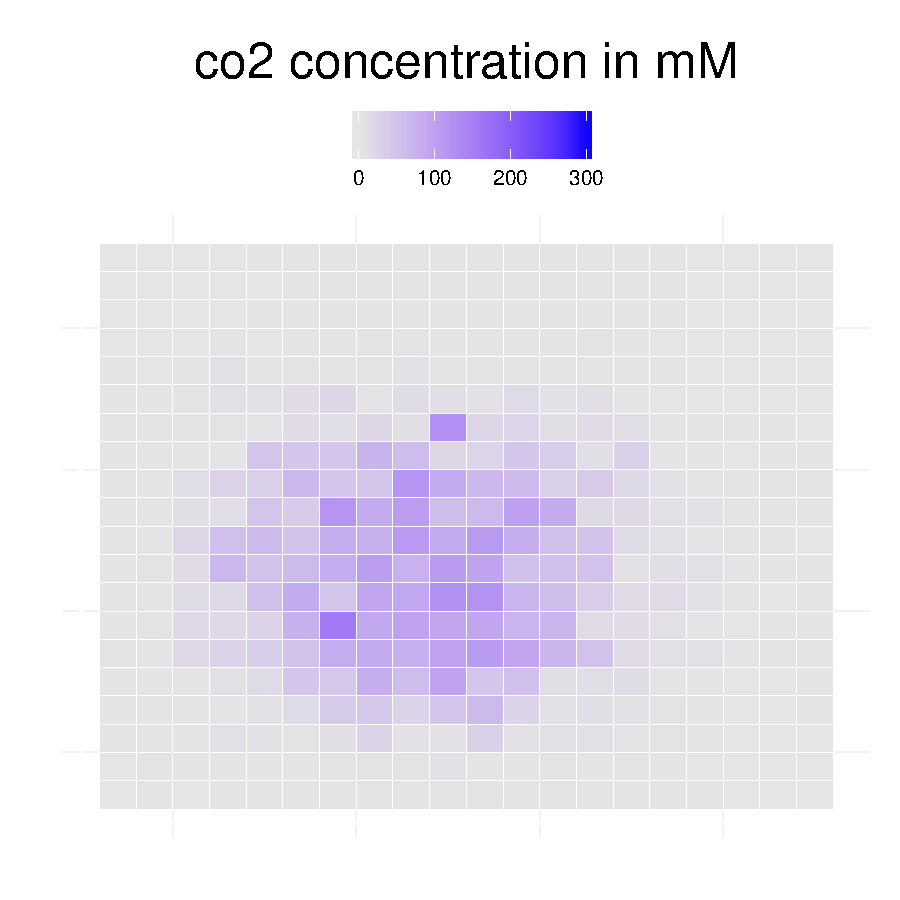
\includegraphics[width=\textwidth]{../results/img/Bcoli_20x20_seed176_co215.pdf}
%  \end{minipage}
%  \begin{minipage}[t]{0.3\textwidth}
%    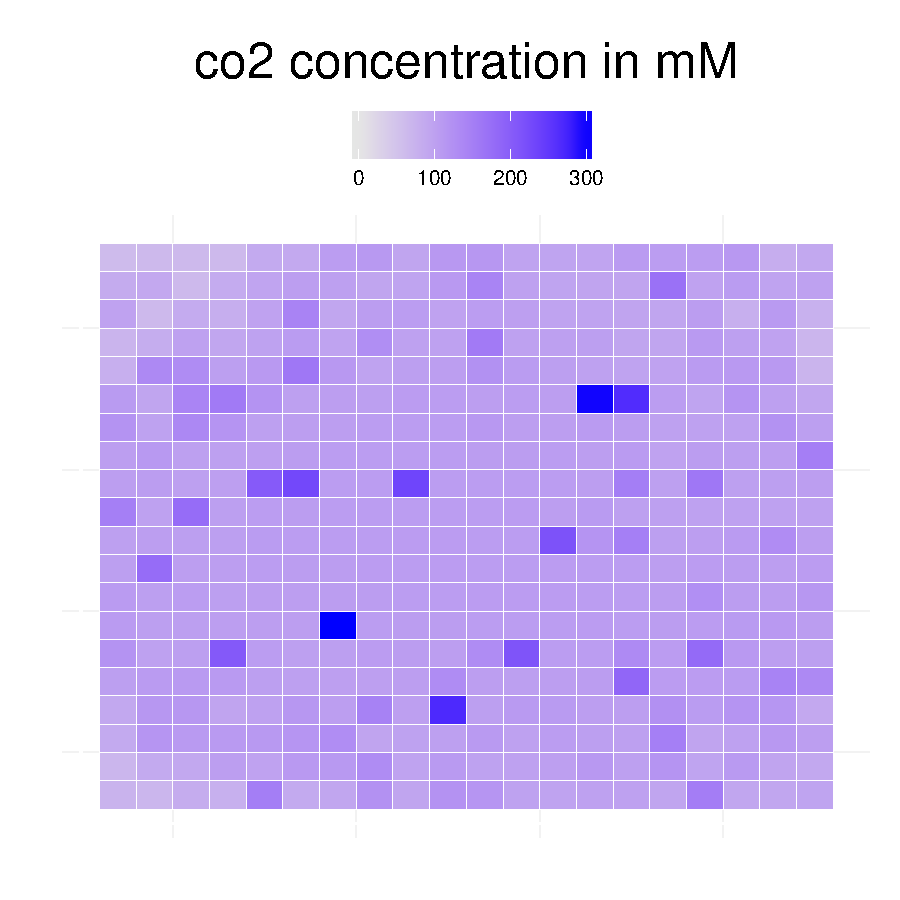
\includegraphics[width=\textwidth]{../results/img/Bcoli_20x20_seed176_co235a.pdf}
%  \end{minipage}
%  }
%  \caption{Population dynamics of the big \emph{E. coli} model on a $20\times20$ grid, with bacterial movement (A) and concentrations of glucose (B), acetate (C) and CO$_2$ (D) (of time step 5, 15 and 35). The seed of the random number generator was set to 176.}
%  \label{fig:ecoligrids}
%\end{figure}

\subsubsection{\textit{Methanosarcina barkeri}}
The \textit{M. barkeri} model was subjected to initial concentrations of methanol as a substrate, to generate a population model and monitor the production/consumption of various metabolites (Figure \hyperref[fig:barkerisg]{\ref{fig:barkerisg}}). In the first time steps methanol was consumed and CO$_2$, methane and water was produced. Compared to water and methane, the production of CO$_2$ was considerably lower.
The doubling time in the exponential phase was estimated as 17 iteration (h).
The population growth reached the stationary phase in approximately 80 iterations (h), after methanol was consumed. In the subsequent death phase no metabolites were produced or consumed. The population died out after 150 iterations.
According the dispersion of the microbes on the grid environment, substrates were consumed and metabolites produced (Figure \hyperref[fig:barkerigrids]{\ref{fig:barkerigrids}}).
\begin{figure}[h!]
  \centering
    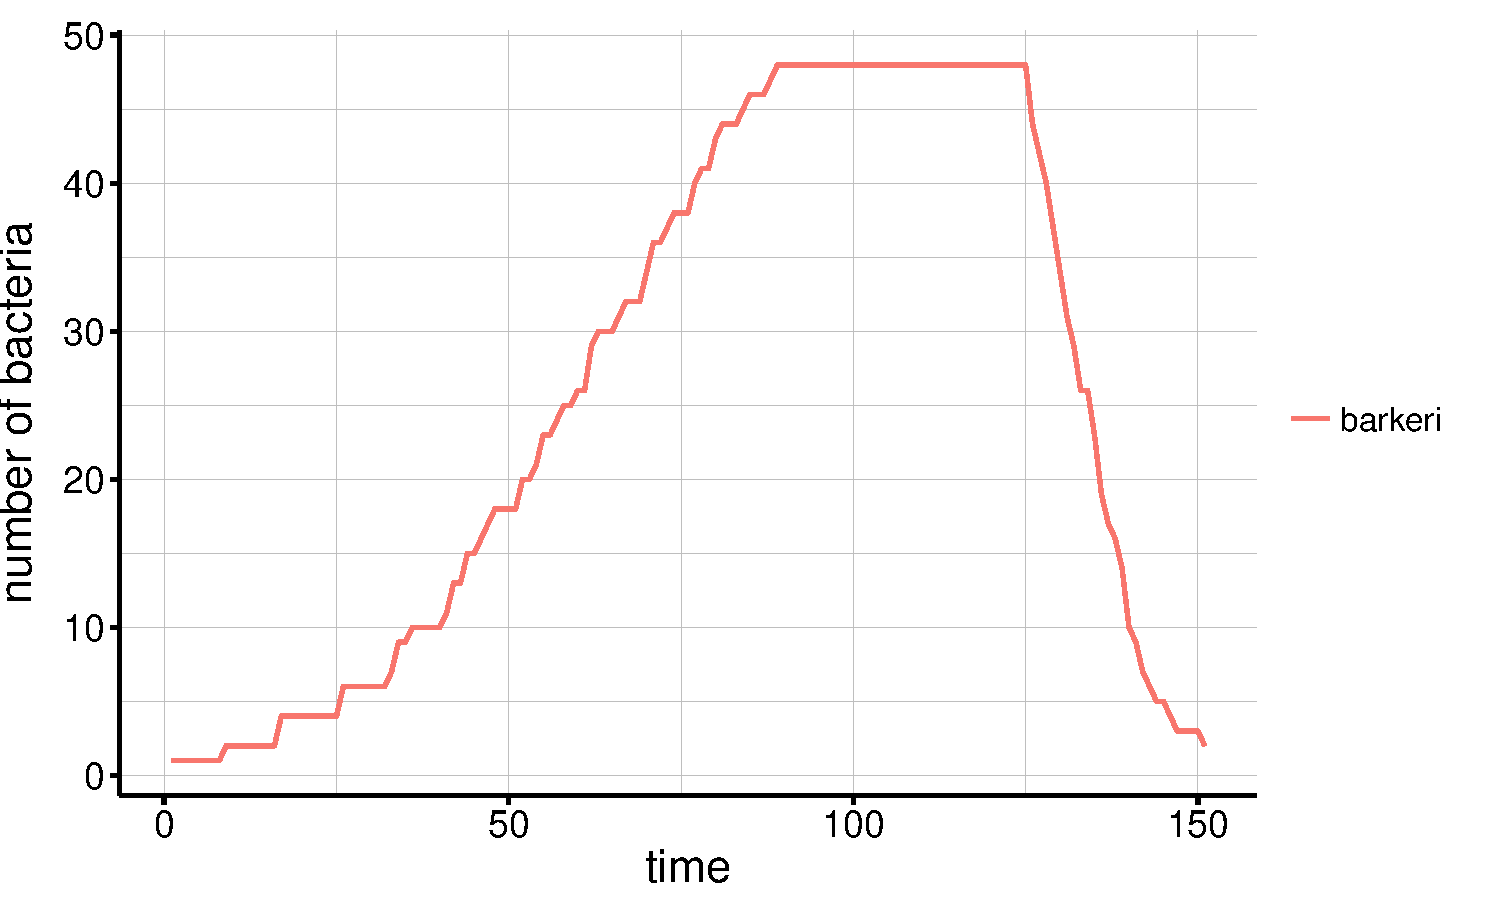
\includegraphics[scale=0.4]{../results/img/barkeri_20x20_seed9659_growth.pdf}
    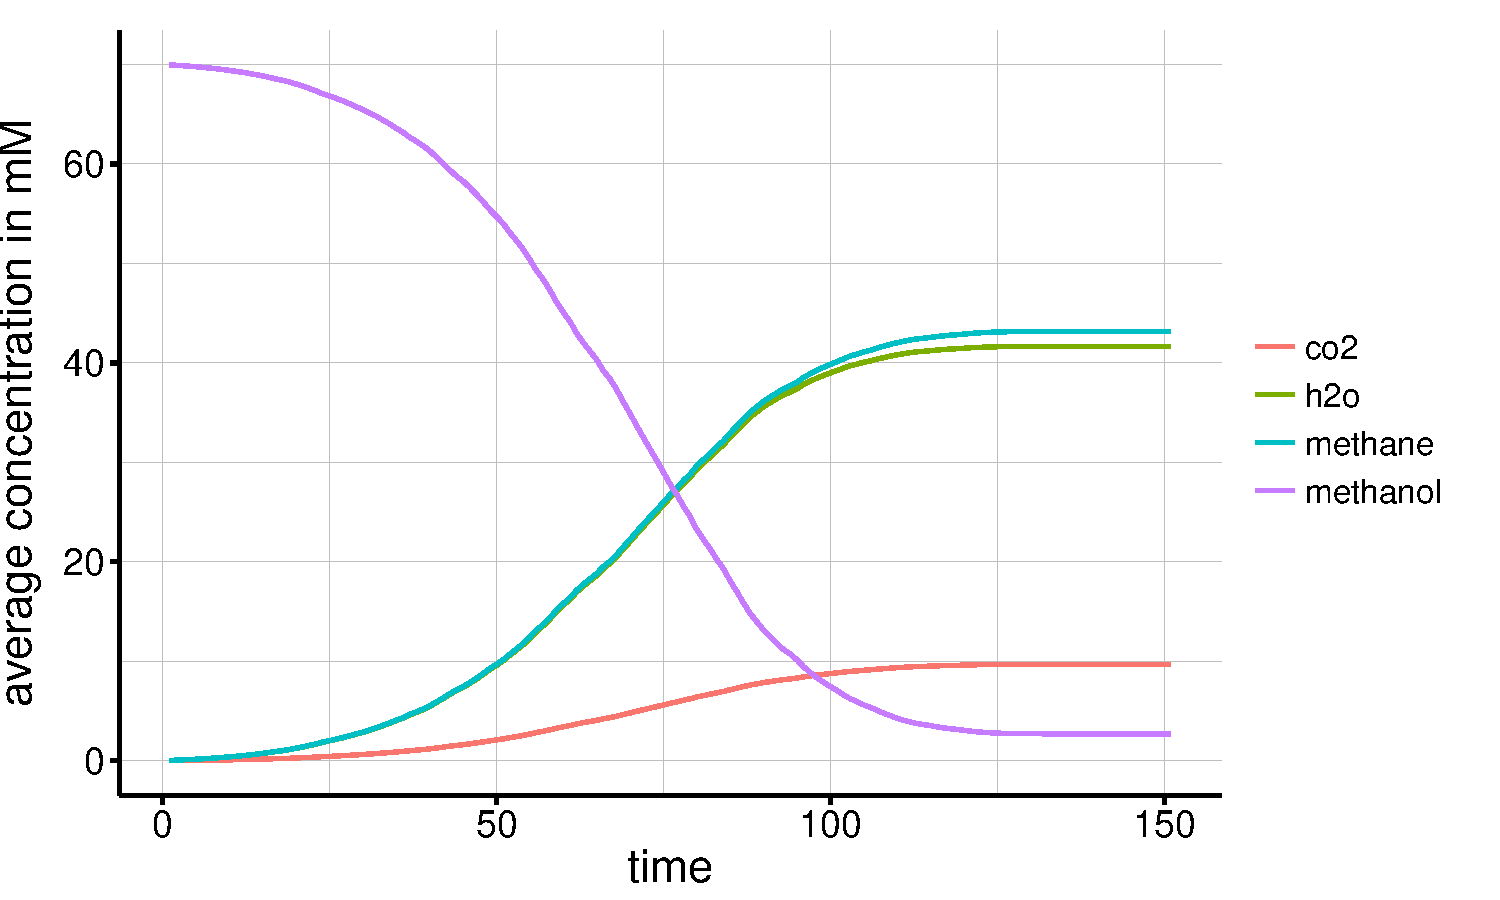
\includegraphics[scale=0.4]{../results/img/barkeri_20x20_seed9659_subs.pdf}
  \caption{Population dynamics of the \emph{M. barkeri} model on a $20\times20$ grid, with bacterial growth (A) and consumption/production of various metabolites (B). An initial concentration of 70\;mmol per grid cell of methanol was added to the environment. The seed of the random number generator was set to 9659.}
  \label{fig:barkerisg}
\end{figure}
\begin{figure}[h!]

  \centering
  \subfigure[]{
    \begin{minipage}[t]{0.3\textwidth}
    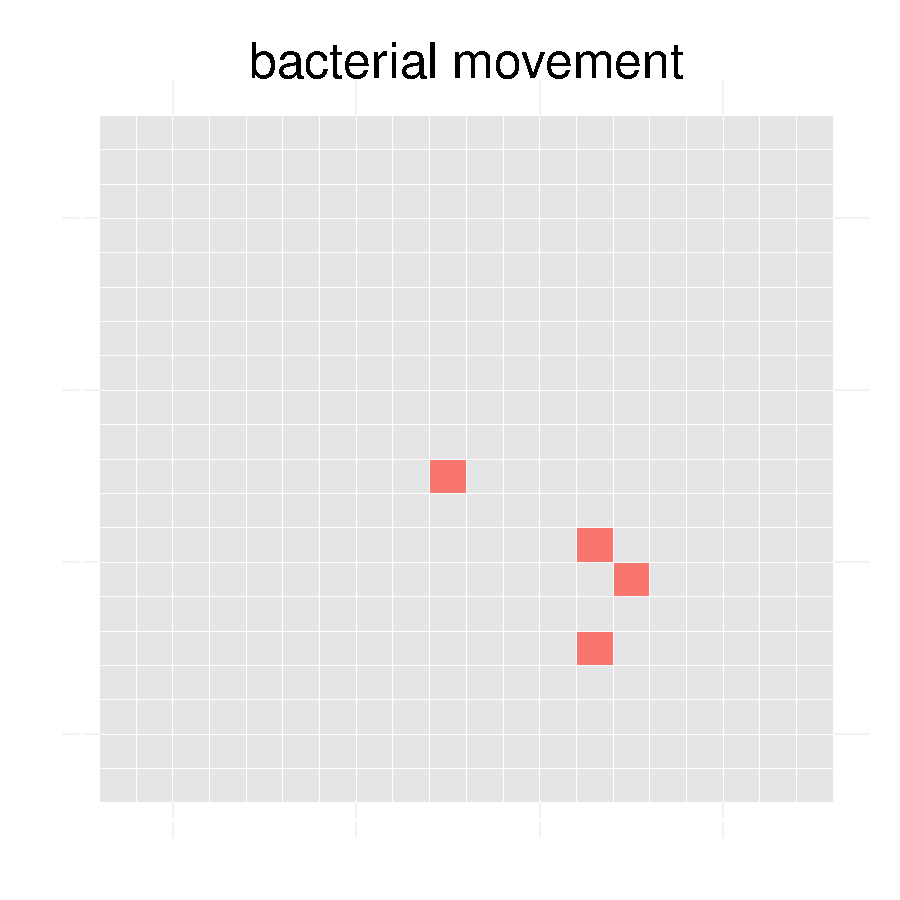
\includegraphics[width=\textwidth]{../results/img/barkeri_20x20_seed9659_bac25.pdf}
  \end{minipage}
  \begin{minipage}[t]{0.3\textwidth}
    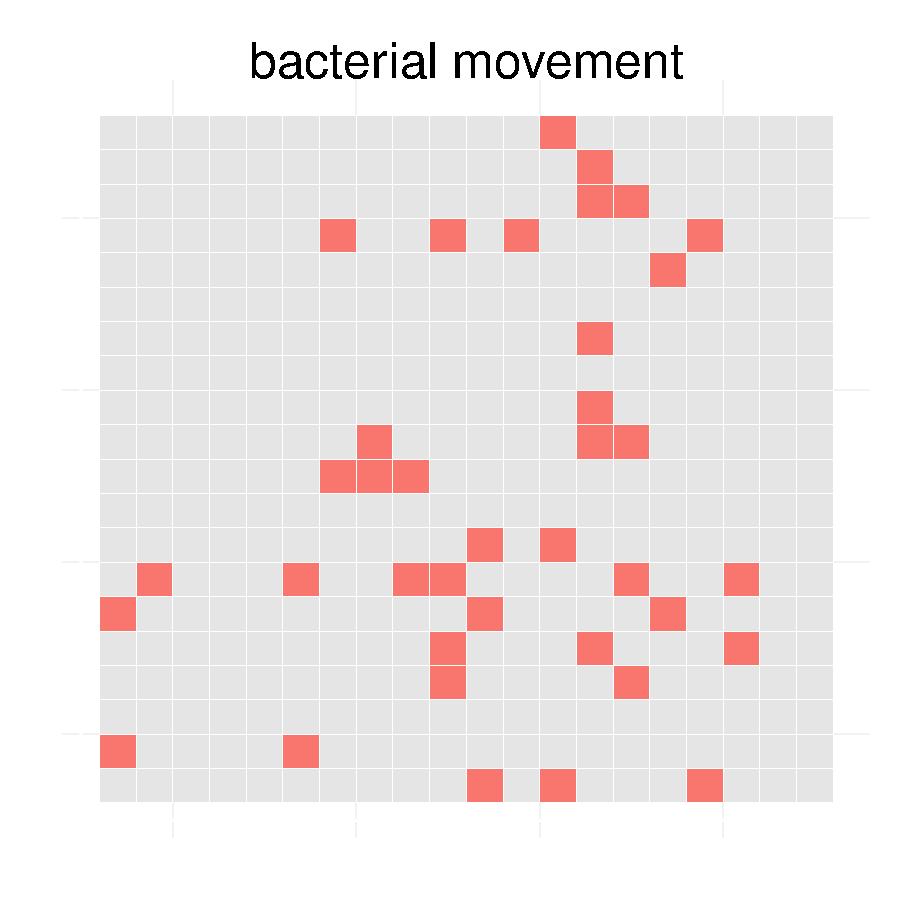
\includegraphics[width=\textwidth]{../results/img/barkeri_20x20_seed9659_bac75.pdf}
  \end{minipage}
  \begin{minipage}[t]{0.3\textwidth}
      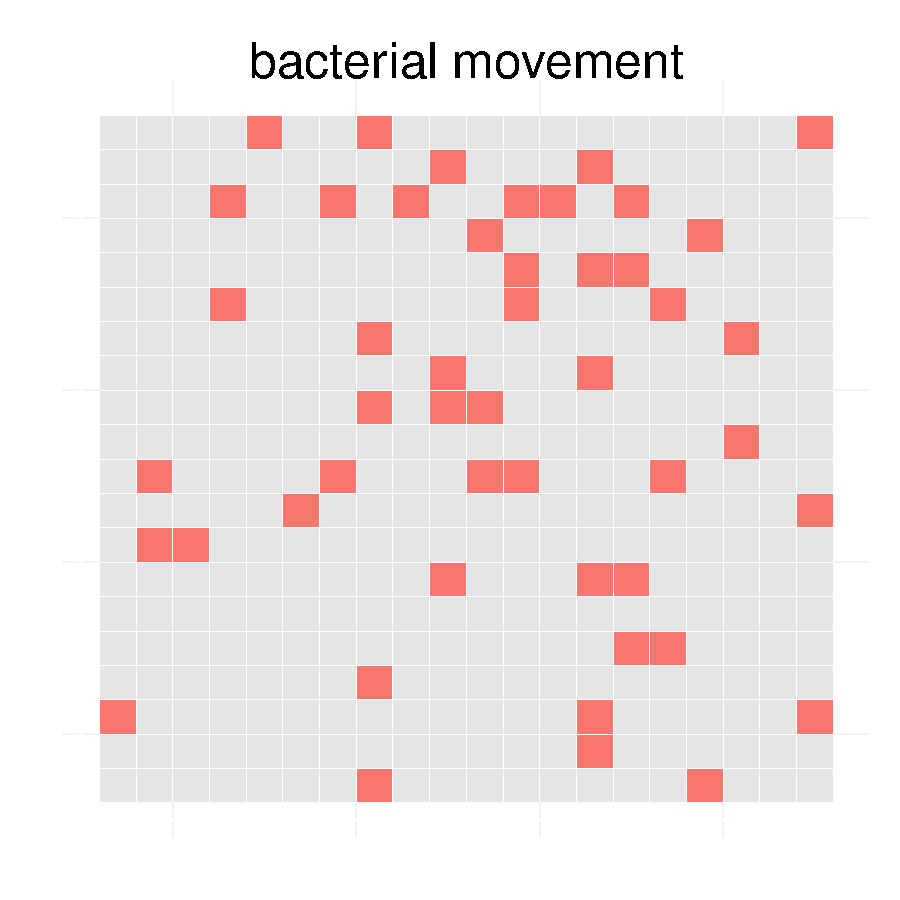
\includegraphics[width=\textwidth]{../results/img/barkeri_20x20_seed9659_bac100.pdf}
  \end{minipage}
  }
  \subfigure[]{
  \begin{minipage}[t]{0.3\textwidth}
    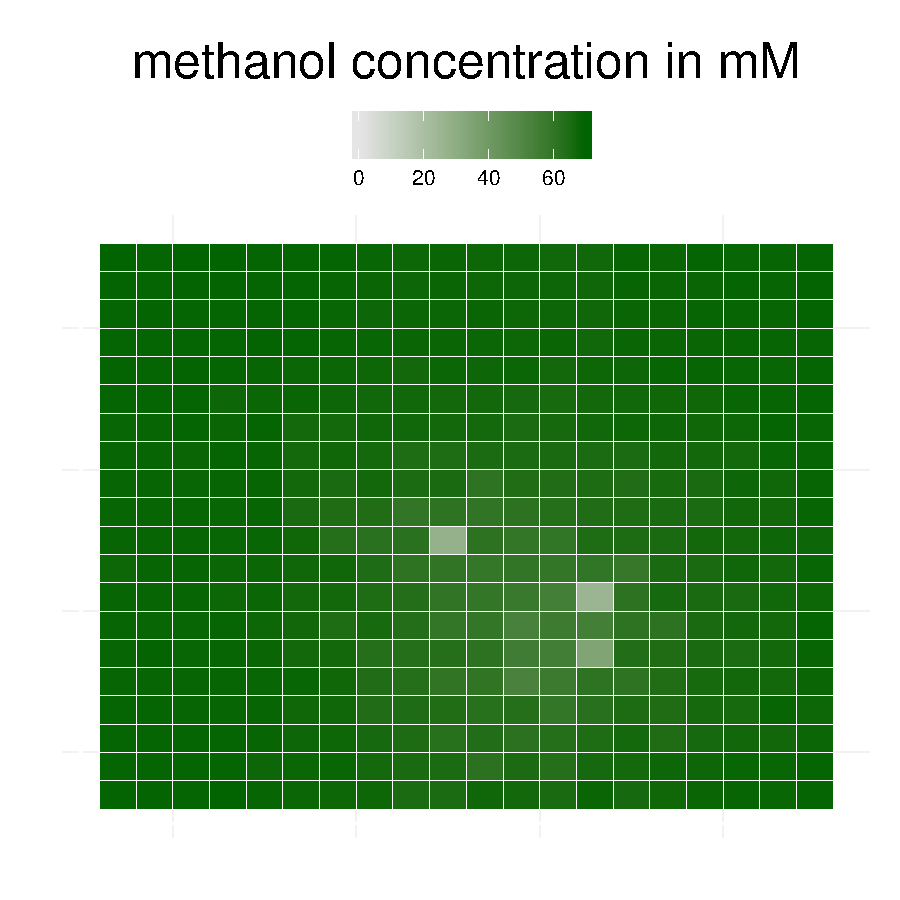
\includegraphics[width=\textwidth]{../results/img/barkeri_20x20_seed9659_meth25.pdf}
  \end{minipage}
  \begin{minipage}[t]{0.3\textwidth}
    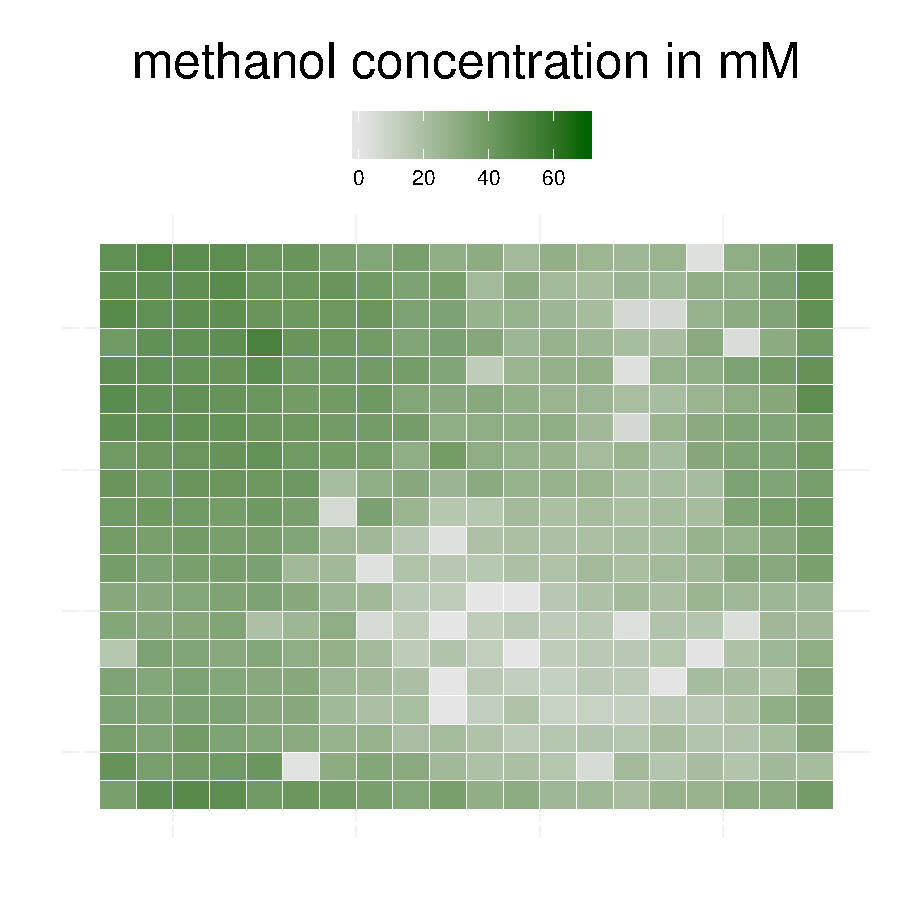
\includegraphics[width=\textwidth]{../results/img/barkeri_20x20_seed9659_meth75.pdf}
  \end{minipage}
  \begin{minipage}[t]{0.3\textwidth}
    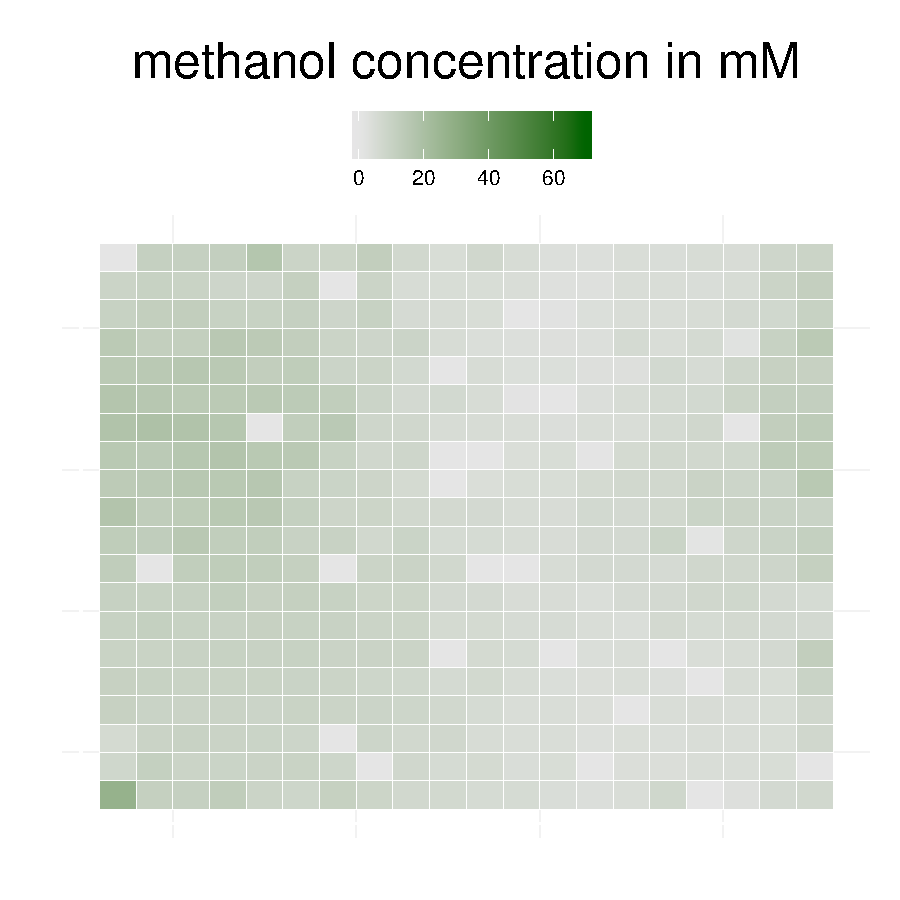
\includegraphics[width=\textwidth]{../results/img/barkeri_20x20_seed9659_meth100.pdf}
  \end{minipage}
  }
  \subfigure[]{
  \begin{minipage}[t]{0.3\textwidth}
    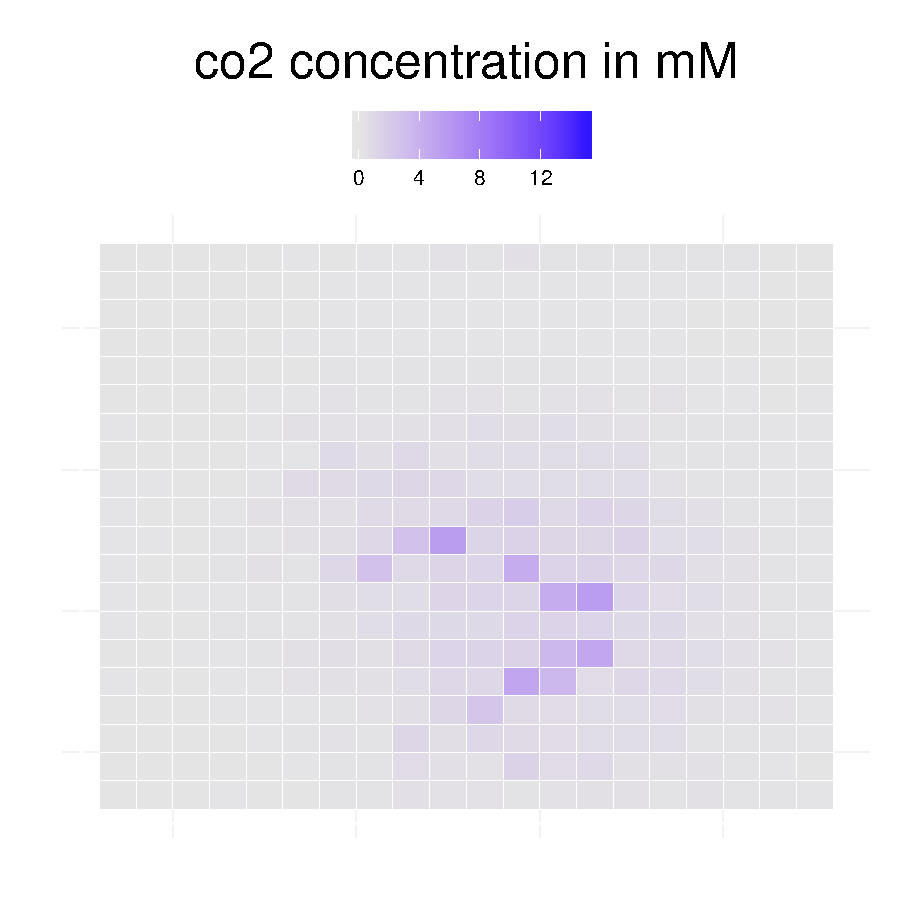
\includegraphics[width=\textwidth]{../results/img/barkeri_20x20_seed9659_co225.pdf}
  \end{minipage}
  \begin{minipage}[t]{0.3\textwidth}
    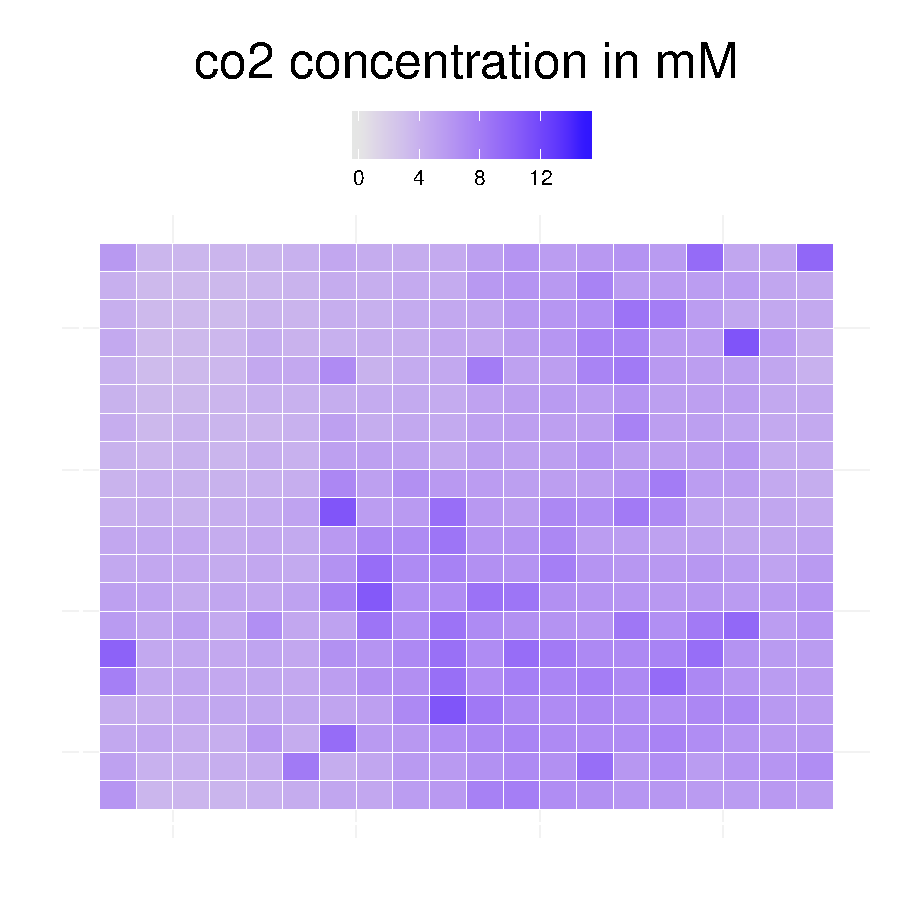
\includegraphics[width=\textwidth]{../results/img/barkeri_20x20_seed9659_co275.pdf}
  \end{minipage}
  \begin{minipage}[t]{0.3\textwidth}
    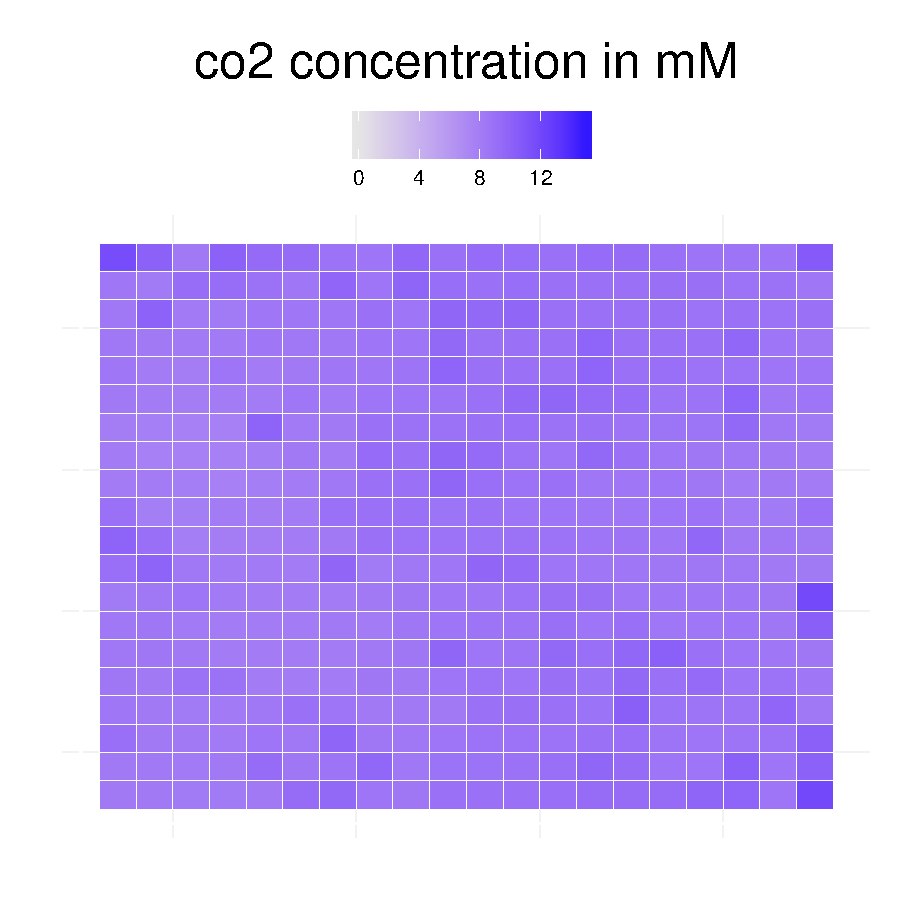
\includegraphics[width=\textwidth]{../results/img/barkeri_20x20_seed9659_co2100.pdf}
  \end{minipage}
  }
  \subfigure[]{
  \begin{minipage}[t]{0.3\textwidth}
    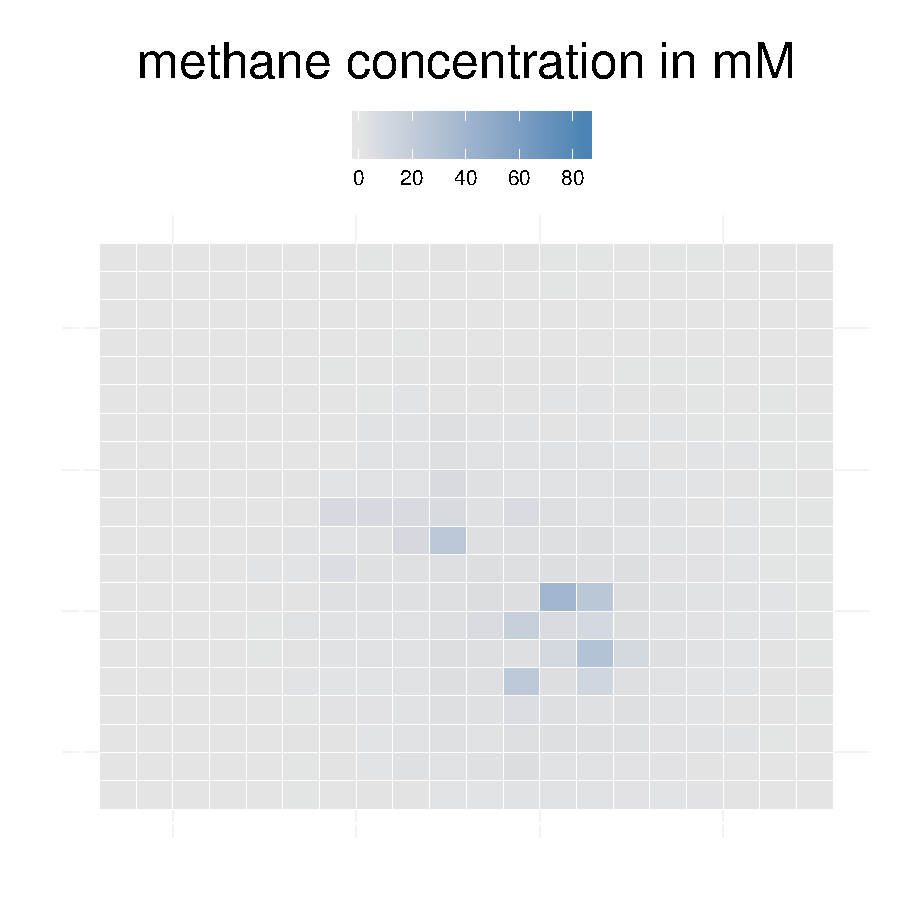
\includegraphics[width=\textwidth]{../results/img/barkeri_20x20_seed9659_methane25.pdf}
  \end{minipage}
  \begin{minipage}[t]{0.3\textwidth}
    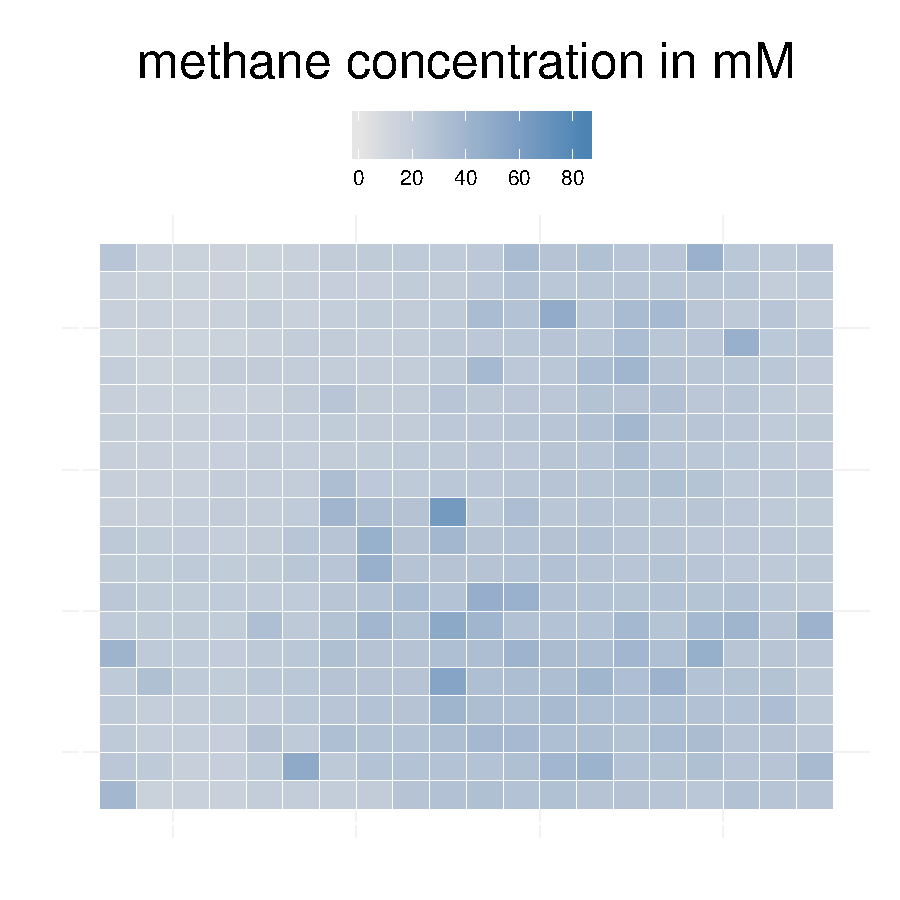
\includegraphics[width=\textwidth]{../results/img/barkeri_20x20_seed9659_methane75.pdf}
  \end{minipage}
  \begin{minipage}[t]{0.3\textwidth}
    \includegraphics[width=\textwidth]{../results/img/barkeri_20x20_seed9659_methane100.pdf}
  \end{minipage}
  }
  \caption{Population dynamics of the \emph{M. barkeri} model on a $20\times20$ grid, with bacterial movement (A) and concentrations of methanol (B), CO$_2$ (C) and methane (D) (of time step 25, 75 and 100). The seed of the random number generator was set to 9659.}
  %\caption{Population and metabolite dynamics of the \emph{M. barkeri} model on a $20\times20$ grid.}
  \label{fig:barkerigrids}
\end{figure}


\subsubsection{\textit{Clostridium beijerinckii}}
The \textit{C. beijerinckii} model was subjected to initial concentrations of glucose as a substrate, to generate a population model and monitor the production/consumption of various metabolites (Figure \hyperref[fig:beijersg]{\ref{fig:beijersg}}). In the first time steps glucose was consumed and hydrogen, C0$_2$, acetate, butyrate and succinate were produced in descending amounts. 
Compared to the other products hydrogen and CO$_2$ were produced much more.
The doubling time in the exponential phase was estimated as 6 iteration (h).
The population growth reached the stationary phase in approximately 45 iterations (h), after glucose was almost consumed. In the subsequent death phase no metabolites were produced or consumed. The population died out after 65 iterations.
According the dispersion of the microbes on the grid environment, substrates were consumed and metabolites produced (Figure \hyperref[fig:beijergrids]{\ref{fig:beijergrids}}).
\begin{figure}[h!]
  \centering
    \includegraphics[scale=0.4]{../results/img/beijerinckii_20x20_seed943_growth.pdf}
    \includegraphics[scale=0.4]{../results/img/beijerinckii_20x20_seed943_subs.pdf}
  \caption{Population dynamics of the \emph{C. beijerinckii} model on a $20\times20$ grid, with bacterial growth (A) and consumption/production of various metabolites (B). An initial concentration of 70\;mmol per grid cell of glucose was added to the environment. The seed of the random number generator was set to 943.}
  \label{fig:beijersg}
\end{figure}
\begin{figure}[h!]
  \centering
  \subfigure[]{
    \begin{minipage}[t]{0.3\textwidth}
    \includegraphics[width=\textwidth]{../results/img/beijerinckii_20x20_seed943_bac20.pdf}
  \end{minipage}
  \begin{minipage}[t]{0.3\textwidth}
    \includegraphics[width=\textwidth]{../results/img/beijerinckii_20x20_seed943_bac40.pdf}
  \end{minipage}
  \begin{minipage}[t]{0.3\textwidth}
    \includegraphics[width=\textwidth]{../results/img/beijerinckii_20x20_seed943_bac50.pdf}
  \end{minipage}
  }
  \subfigure[]{
  \begin{minipage}[t]{0.3\textwidth}
    \includegraphics[width=\textwidth]{../results/img/beijerinckii_20x20_seed943_glc20.pdf}
  \end{minipage}
  \begin{minipage}[t]{0.3\textwidth}
    \includegraphics[width=\textwidth]{../results/img/beijerinckii_20x20_seed943_glc40.pdf}
  \end{minipage}
  \begin{minipage}[t]{0.3\textwidth}
    \includegraphics[width=\textwidth]{../results/img/beijerinckii_20x20_seed943_glc50.pdf}
  \end{minipage}
  }
  \subfigure[]{
  \begin{minipage}[t]{0.3\textwidth}
    \includegraphics[width=\textwidth]{../results/img/beijerinckii_20x20_seed943_h220.pdf}
  \end{minipage}
  \begin{minipage}[t]{0.3\textwidth}
    \includegraphics[width=\textwidth]{../results/img/beijerinckii_20x20_seed943_h240.pdf}
  \end{minipage}
  \begin{minipage}[t]{0.3\textwidth}
    \includegraphics[width=\textwidth]{../results/img/beijerinckii_20x20_seed943_h250.pdf}
  \end{minipage}
  }
  \subfigure[]{
  \begin{minipage}[t]{0.3\textwidth}
    \includegraphics[width=\textwidth]{../results/img/beijerinckii_20x20_seed943_co220.pdf}
  \end{minipage}
  \begin{minipage}[t]{0.3\textwidth}
    \includegraphics[width=\textwidth]{../results/img/beijerinckii_20x20_seed943_co240.pdf}
  \end{minipage}
  \begin{minipage}[t]{0.3\textwidth}
    \includegraphics[width=\textwidth]{../results/img/beijerinckii_20x20_seed943_co250.pdf}
  \end{minipage}
  }
  \caption{Population dynamics of the \emph{C. beijerinckii} model on a $20\times20$ grid, with bacterial movement (A) and concentrations of glucose (B), hydrogen (C) and CO$_2$ (D) (of time step 20, 40 and 50). The seed of the random number generator was set to 943.}
   %\caption{Population and metabolite dynamics of the \emph{C. beijerinckii} model on a $20\times20$ grid.}
  \label{fig:beijergrids}
\end{figure}

\subsection{Mixed communities}
%To study the metabolic interactions of multiple species the individual models described in the previous sections were loaded in the same grid environment.
\subsubsection{\textit{Escherichia coli} \& \textit{Methanosarcina barkeri}}
The joint simulation of the \textit{E. coli} and \textit{M. barkeri} was subjected to initial concentrations of glucose as a substrate for \textit{E. coli} and methanol as a substrate for \textit{M. barkeri}. In the first time steps the respective substrates were consumed and CO$_2$, acetate, ethanol, formate, water and methane were produced (Figure \hyperref[fig:besg]{\ref{fig:besg}}). Acetate was produced as a fermentation product of \textit{E. coli} and consumed by \textit{M. barkeri}. CO$_2$ was produced by \textit{E. coli} and \textit{M. barkeri}. \textit{E. coli} reached the stationary phase in iteration 90.
Since grid space was additionally occupied by \textit{M. barkeri}, the \textit{E. coli} population slightly grew after stationary phase of \textit{M. barkeri} in iteration 125. Both populations died out after iteration 175.
The doubling time in the exponential phase was estimated as 17 iterations (h) for \textit{E. coli} and 12 iterations (h) for \textit{M. barkeri}.
According the dispersion of the microbes on the grid environment, substrates were consumed and metabolites produced (Figure \hyperref[fig:cegrid]{\ref{fig:cegrid}}). The production of methane was found in grid positions occupied by \textit{M. barkeri} and glucose consumption was found in position occupied by \textit{E. coli}. In the later stages of growth acetate was consumed by \textit{M. barkeri}.
\begin{figure}[h!]
  \centering
    \includegraphics[scale=0.4]{../results/img/barkeri_ecoli_20x20_seed4612_growth.pdf}
    \includegraphics[scale=0.4]{../results/img/barkeri_ecoli_20x20_seed4612_subs.pdf}
  \caption{Population dynamics of the joint big \emph{E. coli} and \emph{M. barkeri} model on a $20\times20$ grid, with bacterial growth (A) and consumption/production of various metabolites (B). An initial concentration of 70\;mmol per grid cell of glucose and methanol was added to the environment. The seed of the random number generator was set to 4612.}
  \label{fig:besg}
\end{figure}
\begin{figure}[h!]
  \centering
  \subfigure[]{
    \begin{minipage}[t]{0.3\textwidth}
    \includegraphics[width=\textwidth]{../results/img/barkeri_ecoli_20x20_seed4612_bac60.pdf}
  \end{minipage}
  \begin{minipage}[t]{0.3\textwidth}
    \includegraphics[width=\textwidth]{../results/img/barkeri_ecoli_20x20_seed4612_bac100.pdf}
  \end{minipage}
  \begin{minipage}[t]{0.3\textwidth}
    \includegraphics[width=\textwidth]{../results/img/barkeri_ecoli_20x20_seed4612_bac125.pdf}
  \end{minipage}
  }
  \subfigure[]{
  \begin{minipage}[t]{0.3\textwidth}
    \includegraphics[width=\textwidth]{../results/img/barkeri_ecoli_20x20_seed4612_glc60.pdf}
  \end{minipage}
  \begin{minipage}[t]{0.3\textwidth}
    \includegraphics[width=\textwidth]{../results/img/barkeri_ecoli_20x20_seed4612_glc100.pdf}
  \end{minipage}
  \begin{minipage}[t]{0.3\textwidth}
    \includegraphics[width=\textwidth]{../results/img/barkeri_ecoli_20x20_seed4612_glc125.pdf}
  \end{minipage}
  }
  \subfigure[]{
  \begin{minipage}[t]{0.3\textwidth}
    \includegraphics[width=\textwidth]{../results/img/barkeri_ecoli_20x20_seed4612_ace60.pdf}
  \end{minipage}
  \begin{minipage}[t]{0.3\textwidth}
    \includegraphics[width=\textwidth]{../results/img/barkeri_ecoli_20x20_seed4612_ace100.pdf}
  \end{minipage}
  \begin{minipage}[t]{0.3\textwidth}
    \includegraphics[width=\textwidth]{../results/img/barkeri_ecoli_20x20_seed4612_ace125.pdf}
  \end{minipage}
  }
  \subfigure[]{
  \begin{minipage}[t]{0.3\textwidth}
    \includegraphics[width=\textwidth]{../results/img/barkeri_ecoli_20x20_seed4612_meth60.pdf}
  \end{minipage}
  \begin{minipage}[t]{0.3\textwidth}
    \includegraphics[width=\textwidth]{../results/img/barkeri_ecoli_20x20_seed4612_meth100.pdf}
  \end{minipage}
  \begin{minipage}[t]{0.3\textwidth}
    \includegraphics[width=\textwidth]{../results/img/barkeri_ecoli_20x20_seed4612_meth125.pdf}
  \end{minipage}
  }
  \caption{Population dynamics of the joint big \emph{E. coli} and \emph{M. barkeri} model on a $20\times20$ grid, with bacterial movement (A) and concentrations of glucose (B), acetate (C) and methane (D) (of time step 60, 100 and 125). The seed of the random number generator was set to 4612.}
%  \caption{Population and metabolite dynamics of the joint \emph{E. coli} and \emph{M. barkeri} model.}
  \label{fig:begrid}
\end{figure}

\subsubsection{\textit{Escherichia coli big} \& \textit{Clostridium beijerinckii}}
The joint simulation of the \textit{E. coli} and \textit{C. beijerinckii} was subjected to initial concentrations of glucose as a substrate for both organisms. In the first time steps the substrate was competitively consumed by both species and CO$_2$, acetate, ethanol, butyrate, succinate and hydrogen was produced (Figure \hyperref[fig:cesg]{\ref{fig:cesg}}). In comparison to the other metabolites hydrogen and CO$_2$ had the highest concentrations at the end of the simulation.
Hydrogen, CO$_2$, butyrate and succinate were exclusively produced by \textit{C. beijerinckii}, whereas ethanol was produced by \textit{E. coli}. 
Acetate was produced by both species. \textit{C. beijerinckii} reached the stationary phase at 55 iterations and \textit{E. coli} at 60 iterations. Both organisms died at iteration 80. In the exponential phase \textit{C. beijerinckii} had an approximate duplication time of 8 iterations and \textit{E. coli} of 11 iterations.

According the dispersion of the microbes on the grid environment, substrates were consumed and metabolites produced (Figure \hyperref[fig:cegrid]{\ref{fig:cegrid}}). Hydrogen production was found in \textit{C. beijerinckii} occupied grid positions and ethanol production in \textit{E. coli} occupied positions.
\begin{figure}[h!]
  \centering
    \includegraphics[scale=0.4]{../results/img/ecoli_beijerinckii_20x20_seed5147_growth.pdf}
    \includegraphics[scale=0.4]{../results/img/ecoli_beijerinckii_20x20_seed5147_subs.pdf}
  \caption{Population dynamics of the joint big \emph{E. coli} and \emph{C. beijerinckii} model on a $20\times20$ grid, with bacterial growth (A) and consumption/production of various metabolites (B). An initial concentration of 70\;mmol per grid cell of glucose was added to the environment. The seed of the random number generator was set to 5147.}
  \label{fig:cesg}
\end{figure}
\begin{figure}[h!]
  \centering
  \subfigure[]{
    \begin{minipage}[t]{0.3\textwidth}
    \includegraphics[width=\textwidth]{../results/img/ecoli_beijerinckii_20x20_seed5147_bac25.pdf}
  \end{minipage}
  \begin{minipage}[t]{0.3\textwidth}
    \includegraphics[width=\textwidth]{../results/img/ecoli_beijerinckii_20x20_seed5147_bac55.pdf}
  \end{minipage}
  \begin{minipage}[t]{0.3\textwidth}
    \includegraphics[width=\textwidth]{../results/img/ecoli_beijerinckii_20x20_seed5147_bac65.pdf}
  \end{minipage}
  }
  \subfigure[]{
  \begin{minipage}[t]{0.3\textwidth}
    \includegraphics[width=\textwidth]{../results/img/ecoli_beijerinckii_20x20_seed5147_glc25.pdf}
  \end{minipage}
  \begin{minipage}[t]{0.3\textwidth}
    \includegraphics[width=\textwidth]{../results/img/ecoli_beijerinckii_20x20_seed5147_glc55.pdf}
  \end{minipage}
  \begin{minipage}[t]{0.3\textwidth}
    \includegraphics[width=\textwidth]{../results/img/ecoli_beijerinckii_20x20_seed5147_glc65.pdf}
  \end{minipage}
  }
  \subfigure[]{
  \begin{minipage}[t]{0.3\textwidth}
    \includegraphics[width=\textwidth]{../results/img/ecoli_beijerinckii_20x20_seed5147_h225.pdf}
  \end{minipage}
  \begin{minipage}[t]{0.3\textwidth}
    \includegraphics[width=\textwidth]{../results/img/ecoli_beijerinckii_20x20_seed5147_h255.pdf}
  \end{minipage}
  \begin{minipage}[t]{0.3\textwidth}
    \includegraphics[width=\textwidth]{../results/img/ecoli_beijerinckii_20x20_seed5147_h265.pdf}
  \end{minipage}
  }
  \subfigure[]{
  \begin{minipage}[t]{0.3\textwidth}
    \includegraphics[width=\textwidth]{../results/img/ecoli_beijerinckii_20x20_seed5147_eth25.pdf}
  \end{minipage}
  \begin{minipage}[t]{0.3\textwidth}
    \includegraphics[width=\textwidth]{../results/img/ecoli_beijerinckii_20x20_seed5147_eth55.pdf}
  \end{minipage}
  \begin{minipage}[t]{0.3\textwidth}
    \includegraphics[width=\textwidth]{../results/img/ecoli_beijerinckii_20x20_seed5147_eth65.pdf}
  \end{minipage}
  }
  \caption{Population dynamics of the joint big \emph{E. coli} and \emph{C. beijerinckii} model on a $20\times20$ grid, with bacterial movement (A) and concentrations of glucose (B), hydrogen (C) and ethanol (D) (of time step 25, 55 and 65). The seed of the random number generator was set to 5147.}
  %\caption{Dynamics of the joint \emph{E. coli} and \emph{C. beijerinckii} model on a $20\times20$ grid.}
  \label{fig:cegrid}
\end{figure}

\subsubsection{\textit{Clostridium beijerinckii} \& \textit{Methanosarcina barkeri}}
The joint simulation of the \textit{M. barkeri} and \textit{C. beijerinckii} was subjected to initial concentrations of glucose as a exclusive substrate for \textit{C. beijerinckii}. In the first time steps the substrate was consumed by \textit{C. beijerinckii} and CO$_2$, hydrogen, acetate, butyrate and succinate was produced (Figure \hyperref[fig:cbsg]{\ref{fig:cbsg}}). 
In comparison to the other metabolites hydrogen and CO$_2$ had the highest concentrations at the stationary phase of \textit{C. beijerinckii} reached at approximately 60 iterations. The population of \textit{C. beijerinckii} died out at iteration 80 and \textit{M. barkeri} started growing exponentially by taking the produced hydrogen and CO$_2$ as substrates. 
In the later phases of growth the produced acetate was used as a substrate. The stationary phase of \textit{M. barkeri} was reached at iteration 170. 
During growth \textit{M. barkeri} produced methane and water by consuming CO$_2$ and almost the total hydrogen produced by \textit{C. beijerinckii}. 
In the exponential phase \textit{C. beijerinckii} had an approximate duplication time of 8 iterations and \textit{M. barkeri} of 12 iterations.
According the dispersion of the microbes on the grid environment, substrates were consumed and metabolites produced (Figure \hyperref[fig:cbgrid]{\ref{fig:cbgrid}}). Hydrogen production was found in \textit{C. beijerinckii} occupied grid positions and methane production in \textit{M. barkeri} occupied positions.
\begin{figure}[h!]
  \centering
    \includegraphics[scale=0.4]{../results/img/barkeri_beijerinckii_20x20_seed2942_growth.pdf}
    \includegraphics[scale=0.4]{../results/img/barkeri_beijerinckii_20x20_seed2942_subs.pdf}
  \caption{Population dynamics of the joint \emph{M. barkeri} and \emph{C. beijerinckii} model on a $20\times20$ grid, with bacterial growth (A) and consumption/production of various metabolites (B). An initial concentration of 70\;mmol per grid cell of glucose was added to the environment. The seed of the random number generator was set to 2942.}
  \label{fig:cbsg}
\end{figure}
\begin{figure}[h!]
  \centering
  \subfigure[]{
    \begin{minipage}[t]{0.3\textwidth}
    \includegraphics[width=\textwidth]{../results/img/barkeri_beijerinckii_20x20_seed2942_bac50.pdf}
  \end{minipage}
  \begin{minipage}[t]{0.3\textwidth}
    \includegraphics[width=\textwidth]{../results/img/barkeri_beijerinckii_20x20_seed2942_bac100.pdf}
  \end{minipage}
  \begin{minipage}[t]{0.3\textwidth}
    \includegraphics[width=\textwidth]{../results/img/barkeri_beijerinckii_20x20_seed2942_bac150.pdf}
  \end{minipage}
  }
  \subfigure[]{
  \begin{minipage}[t]{0.3\textwidth}
    \includegraphics[width=\textwidth]{../results/img/barkeri_beijerinckii_20x20_seed2942_glc50.pdf}
  \end{minipage}
  \begin{minipage}[t]{0.3\textwidth}
    \includegraphics[width=\textwidth]{../results/img/barkeri_beijerinckii_20x20_seed2942_glc100.pdf}
  \end{minipage}
  \begin{minipage}[t]{0.3\textwidth}
    \includegraphics[width=\textwidth]{../results/img/barkeri_beijerinckii_20x20_seed2942_glc150.pdf}
  \end{minipage}
  }
  \subfigure[]{
  \begin{minipage}[t]{0.3\textwidth}
    \includegraphics[width=\textwidth]{../results/img/barkeri_beijerinckii_20x20_seed2942_h250.pdf}
  \end{minipage}
  \begin{minipage}[t]{0.3\textwidth}
    \includegraphics[width=\textwidth]{../results/img/barkeri_beijerinckii_20x20_seed2942_h2100.pdf}
  \end{minipage}
  \begin{minipage}[t]{0.3\textwidth}
    \includegraphics[width=\textwidth]{../results/img/barkeri_beijerinckii_20x20_seed2942_h2150.pdf}
  \end{minipage}
  }
  \subfigure[]{
  \begin{minipage}[t]{0.3\textwidth}
    \includegraphics[width=\textwidth]{../results/img/barkeri_beijerinckii_20x20_seed2942_methane50.pdf}
  \end{minipage}
  \begin{minipage}[t]{0.3\textwidth}
    \includegraphics[width=\textwidth]{../results/img/barkeri_beijerinckii_20x20_seed2942_methane100.pdf}
  \end{minipage}
  \begin{minipage}[t]{0.3\textwidth}
    \includegraphics[width=\textwidth]{../results/img/barkeri_beijerinckii_20x20_seed2942_methane150.pdf}
  \end{minipage}
  }
  \caption{Dynamics of the joint \emph{M. barkeri} and \emph{C. beijerinckii} model on a $20\times20$ grid, with bacterial movement (A) and concentrations of glucose (B), hydrogen (C) and methanol (D) (time step 50, 100 and 150). The seed of the random number generator was set to 2942.}
  \label{fig:cbgrid}
  %\caption{Dynamics of the joint \emph{M. barkeri} and \emph{C. beijerinckii} model on a $20\times20$ grid.}
\end{figure}

%\subsection{Spatial and time-wise heterogeneity}
%\subsubsection{Substrate gradients}
%\subsubsection{Delayed bacterial input}


\section{Discussion}
\subsection{General discussion}

\subsubsection{Diffusion and movement}
In agent based modeling two different modes for updating can be distinguished:
A synchronous mode updates all cells simultaneously, i.e. local changes are stored in a temporary copy and will be updated after the computation of all cells.
Contrary to this, a asynchronous mode updates changes immediately (\cite{Matthies2002} p. 92).\\
In our study we implemented for the diffusion rule applied to agents a naive model, which relies on the asynchronous update with randomly chosen cells.
For the diffusion of substrates this method is preferred, because i) synchronous updates would violate the conservation laws by the production of additional metabolite concentrations and ii) non-random asynchronous updates cause a biased diffusion direction \cite{Bandman1999}.
As indicated in Figure \hyperref[fig:diff]{\ref{fig:diff}} the spreading of metabolite concentrations causes the increase of entropy in the system, which is also observed as a physical phenomenon in microbial communities \cite{Wetzel93}.
Additional refinements can be realized with more sofisticated diffusion models such as block-rotation \cite{Bandman1999} or the discrete diffusion model by Grajdeanu \cite{Grajdeanu2007}.
Different diffusion coefficients of certain metabolites could also be included to model the varying dispersal speeds.\\
The bacterial movement was implemented similar to the diffusion model as a random spread on the grid environment (Figure \hyperref[fig:mov]{\ref{fig:mov}}).
Since most bacteria are able to sense the metabolite concentrations in their environment and show a directed motion to the substrate of choice \cite{Francisco13}, the movement model can be refined by interaction of the bacterial agents with the substrates.
A chemotaxis model would also probably allow the observation of more complex behaviours such as the aggregation to certain parts of the grid environment.

\subsubsection{Time consumption}
FBA calculation of substrate exchange can take $2\,min$ per time step for $180$ bacteria of the big \textit{E. coli} model ($1972\times 2382$ metabolites and substrates).
This leads to an overall calculation time of several hours for the \textit{Bcoli} population model.
In comparison to this, the \textit{E. coli} ($77\times 77$) core model needed only $2\,$s per time step for $180$ bacteria.
Almost all of the required time is spent for fba calculation.
For this reason further improvements can be done by:
\begin{enumerate}
  \item Hashing: Implementation of a fba memory table, which saves prior calculations.
  \item Starting base: \textit{lpsolve} offers since version $5.1.05$ the possibility to find a basis according to some guessed vector (old solution).
    With this basis the optimal solution of the optimization problem might be found faster \cite{warmstart}.
\end{enumerate}
We implemented already a first form of hashing, however the speed improvements were so far not quantified and compared. 

\subsection{Population models of single organisms}
All population models show similarities in their growth curves (Figure \hyperref[fig:ecoresg]{\ref{fig:ecoresg}}, \hyperref[fig:ecolisg]{\ref{fig:ecolisg}}, \hyperref[fig:barkerisg]{\ref{fig:barkerisg}} and \hyperref[fig:beijersg]{\ref{fig:beijersg}}).
Roughly, the observed growth can be separated into three phases: the exponential, the stationary and the death phase. Those phases are also observed in experimental studies of microbial growth \cite{Varma1994}.
During the exponential phase all substrates are efficiently used by the fba to accumulate biomass, which is then used for duplication. In the stationary phase almost all substrates were exploited and the fba does not find any feasible solution, which results in the reduction of biomass. Subsequently, bacterial agents are removed, if the biomass is below zero, leading to the death phase.

According to experimental studies \cite{Varma1994}, the time for \emph{E. coli} to reach the stationary phase is about 8\;h, which is in contradiction to the observed time of approximately 39\;h in our study (Figure \hyperref[fig:ecoresg]{\ref{fig:ecoresg}}). This can be explained by the used artificial media composition, which might not be sufficient for an optimal growth.
Moreover, the substrate concentrations were set to not empirically justified arbitrary values. Further refinements of substrate concentrations could thus increase the accuracy of the model to match experimental results. Additionally, the constraints of the used exchange reactions can also be refined to more realistic values.

The observed growth of \emph{E. coli} (Figure \hyperref[fig:ecoresg]{\ref{fig:ecoresg}}) can be explained mainly by the aerobic respiration of glucose:
\[
  \textrm{C}_{6}\textrm{H}_{12}\textrm{O}_{6} + 6\textrm{O}_2 \rightarrow 6\textrm{CO}_{2} + 6 \textrm{H}_{2}\textrm{O}
\]
where one molecule of glucose and 6 molecules of oxygen are consumed to produce 6 molecules of CO$_2$ and water. In accordance to the stochiometry of this reaction more oxygen was consumed by the model compared to glucose (Figure \hyperref[fig:ecolisg]{\ref{fig:ecolisg}}). Additionally, various fermentation products are produced via mixed acid fermentation under aerobic conditions (Figure \hyperref[fig:ecoresg]{\ref{fig:ecoresg}}), which is in concordance to experimental studies \cite{Sunya13}.
In these studies, formate is only produced under anaerobic conditions. Interestingly, the production of formate is observed under aerobic conditions in \emph{E. coli} core, whereas \emph{E. coli} big does not produce formate (Figure \hyperref[fig:ecoresg]{\ref{fig:ecoresg}}).
Furthermore, the smaller \emph{E. coli} core model produces overall more fermentation products relative to CO$_2$. This can be explained by the additional pathways present in the more representative larger \emph{E. coli} model, which make the complete mineralization of glucose to CO$_2$ more preferable in the fba optimization.
Since the complete mineralization of glucose would be even more preferable in the larger \emph{E. coli} model, the applied uptake constraints (Table \hyperref[ab:const]{\ref{tab:const}}) were set to allow the production of fermentation products.

The growth of \emph{M. barkeri} (Figure \hyperref[fig:barkerisg]{\ref{fig:barkerisg}}) can be explained by the fermentation of methanol to methane with
\[
  4\textrm{CH}_{3}\textrm{OH} \rightarrow 3\textrm{CH}_{4} + \textrm{CO}_{2} + 2\textrm{H}_{2}\textrm{O}
\]
where 4 molecules of methanol are consumed to produce 3 molecules of methane, 2 of water and 1 molecule CO$_2$.
The stochiometry of this reaction was fulfilled by the higher production of methane compared to CO$_2$ (Figure \hyperref[fig:barkerisg]{\ref{fig:barkerisg}}). However, water was, similar to methane, produced in high amounts, which can be explained by additional reactions in the model, which might lead to water production.
In experimental studies the stationary phase of \emph{M. barkeri} under the consumption of methanol is reached after 72\;h \cite{Hippe79} which is in concordance to our observed time of approximately 80\;h. 

\textit{C. beijerinckii} is able to convert glucose to various fermentation products \cite{Ezeji03} via butyrate fermentation. To remove reducing equivalents hydrogen is formed, which is also observed in our model (Figure \hyperref[fig:beijersg]{\ref{fig:beijersg}}). The time for \textit{C. beijerinckii} to reach the stationary phase with glucose as a substrate was experimentally determined to approximately 60\;h \cite{Ezeji03}, which is in contradiction to the observed time of 40\;h (Figure \hyperref[fig:beijersg]{\ref{fig:beijersg}}). To match the experimental results the constraints of the exchange reaction can be refined.

Growth deviations (especially doubling time) have to be checked with multiple runs and a wide range of circumstances to guarantee more representative results.

\subsection{Interactions in mixed communities}
Since \textit{M. barkeri} can also utilize hydrogen and CO$_2$ for methane production and \textit{C. beijerinckii} is able to produce those metabolites, both organisms are good candidates to study inter-species hydrogen transfer and syntrophy.
Furthermore, co-culture studies on \textit{M. barkeri} with hydrogen producing microbes \cite{Winter79} have demonstrated the capabilities of \textit{M. barkeri} to interact with other organisms.

In our mixed community model (Figure \hyperref[fig:cbsg]{\ref{fig:cbsg}}) we could observe the usage of \textit{C. beijerinckii}'s produced hydrogen and CO$_2$ by \textit{M. barkeri}. However, in contrast to experimental observations showing the parallel growth of both organisms \cite{Winter79}, we observed a delayed growth of \textit{M. barkeri} after the death of \textit{C. beijerinckii} (Figure \hyperref[fig:cbsg]{\ref{fig:cbsg}}). This can be explained by the limited space on the grid environment, which favoured the initial growth of \textit{C. beijerinckii}, since enough substrates were available. Consequently, \textit{M. barkeri} did not have enough space to duplicate and could only spread after the other organism died out (Figure \hyperref[fig:cbgrid]{\ref{fig:cbgrid}}). 
Nevertheless, \textit{M. barkeri} was still able to survive, due to the hydrogen and CO$_2$ support by \textit{C. beijerinckii}.
With the production of \textit{M. barkeri}'s essential metabolites, \textit{C. beijerinckii} thus shaped the environment of the other organism.

In the co-culture of \textit{C. beijerinckii} with \textit{E. coli} we observed competitive interactions, where both organisms competed for the same substrate. In this context, \textit{C. beijerinckii} was able to outcompete the other bacterium with an overall higher growth (Figure \hyperref[fig:cegrid]{\ref{fig:cegrid}}). \textit{E. coli} was not able to show high growth rates, since the main substrate was consumed by the competitor.

These results might indicate a more efficient anaerobic degradation by \textit{C. beijerinckii} compared to \textit{E. coli}.
Another explanation can be the pure chance of \textit{C. beijerinckii} having better starting conditions, which lead to a higher growth (positive feedback).
Further experimental co-culture studies might validate this observation.

In the co-culture of \textit{M. barkeri} with \textit{E. coli} we observed space competitive effects, in which the space was not sufficient to harbour both organisms at their stationary phase (Figure \hyperref[fig:begrid]{\ref{fig:begrid}}). The growth curves of both species were similar to each other, which speaks for no competitive metabolic interactions as observed in the \textit{C. beijerinckii}, \textit{E. coli} joint model (Figure \hyperref[fig:cesg]{\ref{fig:cesg}}).
Moreover, \textit{M. barkeri} was able to utilize acetate produced by \textit{E. coli} (Figure \hyperref[fig:besg]{\ref{fig:besg}}).

\subsection{Conclusions \& outlook}
In the last years a lot of work has been done to build up models for single organisms \cite{lewis2012}.
This models are capable to reproduce experimental results and permit even quantitative phenotypic predictions \cite{mccloskey}.
Recently, voices were being raised to point out the future direction of research on community systems biology:
\begin{quote}
,,We anticipate that, through the use of bottom-up approaches supplemented with meta-omics data, the success of systems biology for individual organisms will now be extended to communities of organisms, and in particular to microbial communities.'' \cite{cosys}
\end{quote}
We implemented such a bottom up approach in our agent based model, which uses the established strength of individual models to simulate metabolic interactions and even syntrophy between communities of \textit{in silico} species.



\printbibliography 

\end{document}


\begin{items}
  \item
\end{items}
\begin{enumerate}
  \item
\end{enumerate}
